% Template for PLoS
% Version 3.6 Aug 2022
%
% % % % % % % % % % % % % % % % % % % % % %
%
% -- IMPORTANT NOTE
%
% This template contains comments intended 
% to minimize problems and delays during our production 
% process. Please follow the template instructions
% whenever possible.
%
% % % % % % % % % % % % % % % % % % % % % % % 
%
% Once your paper is accepted for publication, 
% PLEASE REMOVE ALL TRACKED CHANGES in this file 
% and leave only the final text of your manuscript. 
% PLOS recommends the use of latexdiff to track changes during review, as this will help to maintain a clean tex file.
% Visit https://www.ctan.org/pkg/latexdiff?lang=en for info or contact us at latex@plos.org.
%
%
% There are no restrictions on package use within the LaTeX files except that no packages listed in the template may be deleted.
%
% Please do not include colors or graphics in the text.
%
% The manuscript LaTeX source should be contained within a single file (do not use \input, \externaldocument, or similar commands).
%
% % % % % % % % % % % % % % % % % % % % % % %
%
% -- FIGURES AND TABLES
%
% Please include tables/figure captions directly after the paragraph where they are first cited in the text.
%
% DO NOT INCLUDE GRAPHICS IN YOUR MANUSCRIPT
% - Figures should be uploaded separately from your manuscript file. 
% - Figures generated using LaTeX should be extracted and removed from the PDF before submission. 
% - Figures containing multiple panels/subfigures must be combined into one image file before submission.
% For figure citations, please use "Fig" instead of "Figure".
% See http://journals.plos.org/plosone/s/figures for PLOS figure guidelines.
%
% Tables should be cell-based and may not contain:
% - spacing/line breaks within cells to alter layout or alignment
% - do not nest tabular environments (no tabular environments within tabular environments)
% - no graphics or colored text (cell background color/shading OK)
% See http://journals.plos.org/plosone/s/tables for table guidelines.
%
% For tables that exceed the width of the text column, use the adjustwidth environment as illustrated in the example table in text below.
%
% % % % % % % % % % % % % % % % % % % % % % % %
%
% -- EQUATIONS, MATH SYMBOLS, SUBSCRIPTS, AND SUPERSCRIPTS
%
% IMPORTANT
% Below are a few tips to help format your equations and other special characters according to our specifications. For more tips to help reduce the possibility of formatting errors during conversion, please see our LaTeX guidelines at http://journals.plos.org/plosone/s/latex
%
% For inline equations, please be sure to include all portions of an equation in the math environment.  For example, x$^2$ is incorrect; this should be formatted as $x^2$ (or $\mathrm{x}^2$ if the romanized font is desired).
%
% Do not include text that is not math in the math environment. For example, CO2 should be written as CO\textsubscript{2} instead of CO$_2$.
%
% Please add line breaks to long display equations when possible in order to fit size of the column. 
%
% For inline equations, please do not include punctuation (commas, etc) within the math environment unless this is part of the equation.
%
% When adding superscript or subscripts outside of brackets/braces, please group using {}.  For example, change "[U(D,E,\gamma)]^2" to "{[U(D,E,\gamma)]}^2". 
%
% Do not use \cal for caligraphic font.  Instead, use \mathcal{}
%
% % % % % % % % % % % % % % % % % % % % % % % % 
%
% Please contact latex@plos.org with any questions.
%
% % % % % % % % % % % % % % % % % % % % % % % %

\documentclass[10pt,letterpaper]{article}
\usepackage[top=0.85in,left=2.75in,footskip=0.75in]{geometry}

% amsmath and amssymb packages, useful for mathematical formulas and symbols
\usepackage{amsmath,amssymb}

% Use adjustwidth environment to exceed column width (see example table in text)
\usepackage{changepage}

% textcomp package and marvosym package for additional characters
\usepackage{textcomp,marvosym}

% cite package, to clean up citations in the main text. Do not remove.
\usepackage{cite}

% Use nameref to cite supporting information files (see Supporting Information section for more info)
\usepackage{nameref,hyperref}
%DJM: add this unless instructed otherwise:
\hypersetup{colorlinks,linkcolor=blue,citecolor=blue,urlcolor=blue}



% line numbers
\usepackage[right]{lineno}

% ligatures disabled
\usepackage[nopatch=eqnum]{microtype}
\DisableLigatures[f]{encoding = *, family = * }

% color can be used to apply background shading to table cells only
\usepackage[table]{xcolor}

% array package and thick rules for tables
\usepackage{array}

% create "+" rule type for thick vertical lines
\newcolumntype{+}{!{\vrule width 2pt}}

% create \thickcline for thick horizontal lines of variable length
\newlength\savedwidth
\newcommand\thickcline[1]{%
  \noalign{\global\savedwidth\arrayrulewidth\global\arrayrulewidth 2pt}%
  \cline{#1}%
  \noalign{\vskip\arrayrulewidth}%
  \noalign{\global\arrayrulewidth\savedwidth}%
}

% \thickhline command for thick horizontal lines that span the table
\newcommand\thickhline{\noalign{\global\savedwidth\arrayrulewidth\global\arrayrulewidth 2pt}%
\hline
\noalign{\global\arrayrulewidth\savedwidth}}


% Remove comment for double spacing
\usepackage{setspace} 
\doublespacing

% Text layout
\raggedright
\setlength{\parindent}{0.5cm}
\textwidth 5.25in 
\textheight 8.75in

% Bold the 'Figure #' in the caption and separate it from the title/caption with a period
% Captions will be left justified
\usepackage[aboveskip=1pt,labelfont=bf,labelsep=period,justification=raggedright,singlelinecheck=off]{caption}
\renewcommand{\figurename}{Fig}

% Use the PLoS provided BiBTeX style
\bibliographystyle{plos2015}

% Remove brackets from numbering in List of References
\makeatletter
\renewcommand{\@biblabel}[1]{\quad#1.}
\makeatother



% Header and Footer with logo
\usepackage{lastpage,fancyhdr,graphicx}
\usepackage{epstopdf}
%\pagestyle{myheadings}
\pagestyle{fancy}
\fancyhf{}
%\setlength{\headheight}{27.023pt}
%\lhead{\includegraphics[width=2.0in]{PLOS-submission.eps}}
\rfoot{\thepage/\pageref{LastPage}}
\renewcommand{\headrulewidth}{0pt}
\renewcommand{\footrule}{\hrule height 2pt \vspace{2mm}}
\fancyheadoffset[L]{2.25in}
\fancyfootoffset[L]{2.25in}
\lfoot{\today}

%% Include all macros below

\newcommand{\lorem}{{\bf LOREM}}
\newcommand{\ipsum}{{\bf IPSUM}}

%% END MACROS SECTION

%% add other packages
\usepackage[utf8]{inputenc} % allow utf-8 input
\usepackage[T1]{fontenc}    % use 8-bit T1 fonts
\usepackage{url}            % simple URL typesetting
\usepackage{booktabs}       % professional-quality tables
\usepackage{amsfonts}       % blackboard math symbols
\usepackage{nicefrac}       % compact symbols for 1/2, etc.
\usepackage{lipsum}
%% end 

% lists
\makeatletter
\newcommand{\blist}[1]{\begin{enumerate}[label=\roman*.]\label{list:#1}}
\newcommand{\elist}{\end{enumerate}}
\makeatother

%% user-defined math notations/definitions
\newcommand{\R}{\texttt{R}}
\newcommand{\cpp}{\texttt{C++}}
\newcommand{\fr}[1]{\frac{1}{#1}}
\newcommand{\lr}[1]{\left(#1\right)}
\newcommand{\norm}[1]{\left\lVert #1 \right\rVert}
\newcommand{\abs}[1]{\left\lvert #1 \right\rvert}
\newcommand{\snorm}[1]{\lVert #1 \rVert}
\DeclareMathOperator*{\Lambert}{\mathrm{Lambert}_0}
\DeclareMathOperator*{\diag}{diag}
\DeclareMathOperator*{\argmin}{argmin}
\newcommand{\Argmin}[1]{\underset{#1}{\argmin\ }}
\DeclareMathOperator*{\argmax}{argmax}
\newcommand{\Argmax}[1]{\underset{#1}{\argmax\ }}
\def\sumN{\sum_{i=1}^n}
\def\RtEstim{\texttt{RtEstim}}
\def\EpiEstim{\texttt{EpiEstim}}
\def\EpiLPS{\texttt{EpiLPS}}
\def\EpiFilter{\texttt{EpiFilter}}
\def\EpiNow2{\texttt{EpiNow2}}
% binary relations
\def\condind{{\perp\!\!\!\perp}} %independence/conditional independence
\def\equdist{\stackrel{\text{\rm\tiny d}}{=}} %equal in distribution
\def\equas{\stackrel{\text{\rm\tiny a.s.}}{=}} %equal almost surely
\def\simiid{\sim_{\mbox{\tiny iid}}} %sampled i.i.d
% common vectors and matrices
\def\onevec{\mathbf{1}}
\def\iden{\mathbf{I}} % identity matrix
\def\supp{\text{\rm supp}}
\def\gDeltakk{\Delta^{(k+1)}}
\def\gDeltakkX{\Delta^{(x,k+1)}}
\def\gDeltak{\Delta^{(k)}}
\def\gDeltakX{\Delta^{(x,k)}}
\def\gDelta{\Delta^{(1)}}
\def\gDeltaX{\Delta^{(x,1)}}
\def\gDkk{D^{(k+1)}}
\def\gDk{D^{(k)}}
\def\gD1{D^{(1)}}
\def\Dxk{D^{(x,k)}}
\def\Dxkk{D^{(x,k+1)}}
\def\tDxk{\tilde{D}^{(x,k+1)}}
\def\Var{\mathrm{Var}}
\def\bfp{\mathbf{p}}
\def\bfx{\mathbf{x}}
\def\bfy{\mathbf{y}}
\def\bbE{\mathbb{E}}
\def\calR{\mathcal{R}}
\def\bbN{\mathbb{N}}
\def\bbR{\mathbb{R}}
\def\bbP{\mathbb{P}}
\def\bbZ{\mathbb{Z}}
\renewcommand{\top}{\mathsf{T}}
\def\diff{\mathsf{d}}
\def\th{^{\textnormal{th}}}
\def\first{$1^{\textnormal{st}}$}
\def\second{$2^{\textnormal{nd}}$}
\def\third{$3^{\textnormal{nd}$}}
%% END math definitions/notations

%% user-defined reference structures
\newcommand{\citep}[1]{\cite{#1}}
\renewcommand{\eqref}[1]{Eq~(\ref{#1})}
\renewcommand{\figureautorefname}{Fig}
%\renewcommand{\sectionautorefname}{Section}
%% END reference structures
\usepackage[final]{pdfpages}

\begin{document}
\vspace*{0.2in}

% Title must be 250 characters or less.
\begin{flushleft}
{\Large
\textbf\newline{RtEstim: Effective reproduction number estimation with trend filtering} % Please use "sentence case" for title and headings (capitalize only the first word in a title (or heading), the first word in a subtitle (or subheading), and any proper nouns).
}
\newline
% Insert author names, affiliations and corresponding author email (do not include titles, positions, or degrees).
\\
Jiaping Liu\textsuperscript{1*},
Zhenglun Cai\textsuperscript{2},
Paul Gustafson\textsuperscript{1},
Daniel J. McDonald\textsuperscript{1}
\\
\bigskip
\textbf{1} Department of Statistics, The University of British Columbia, Vancouver, British Columbia, Canada

\textbf{2} Centre for Health Evaluation and Outcome Sciences, The University of British Columbia, Vancouver, British Columbia, Canada
\\

\bigskip

% Insert additional author notes using the symbols described below. Insert symbol callouts after author names as necessary.
% 
% Remove or comment out the author notes below if they aren't used.
%
% Primary Equal Contribution Note
%\Yinyang These authors contributed equally to this work.

% Additional Equal Contribution Note
% Also use this double-dagger symbol for special authorship notes, such as senior authorship.
%\ddag These authors also contributed equally to this work.

% Current address notes
%\textcurrency Current Address: Department of Statistics, The University of British Columbia, Vancouver, British Columbia, Canada % change symbol to "\textcurrency a" if more than one current address note
% \textcurrency b Insert second current address 
% \textcurrency c Insert third current address

% Deceased author note
%\dag Deceased

% Group/Consortium Author Note
%\textpilcrow Membership list can be found in the Acknowledgments section.

% Use the asterisk to denote corresponding authorship and provide email address in note below.
* jiaping.liu@stat.ubc.ca

\end{flushleft}
% Please keep the abstract below 300 words
\section*{Abstract}

To understand the transmissibility and spread of infectious diseases,
epidemiologists turn to estimates of the effective reproduction number.
While many estimation approaches exist, their utility may be limited. 
Challenges of surveillance data collection, model assumptions
that are unverifiable with data alone, and 
computationally inefficient frameworks are critical limitations for many
existing approaches. We propose a discrete spline-based approach 
\RtEstim\ that solves a convex optimization problem---Poisson trend filtering---using the proximal Newton method. It produces a locally adaptive 
estimator for effective reproduction number estimation with heterogeneous 
smoothness. \RtEstim\ remains accurate even under some process 
misspecifications and is computationally efficient, even for large-scale 
data. The implementation is easily accessible in a lightweight \R\ 
package \href{https://dajmcdon.github.io/rtestim/index.html}{\texttt{rtestim}}.

% {\bf Keywords:} discrete splines $|$ piecewise polynomials $|$
% PLOS CB doesn't use these, seemingly

% Please keep the Author Summary between 150 and 200 words
% Use first person. PLOS ONE authors please skip this step. 
% Author Summary not valid for PLOS ONE submissions.   
\section*{Author summary}

Effective reproduction number estimation presents many challenges due to data
collection, modelling assumptions, and computational burden. Such limitations
hinder the accurate estimation of the effective reproduction number. Our
motivation is to develop a model that produces accurate estimates, is robust to
model misspecification, and is straightforward to use and computationally
efficient, even for large counts and long time periods. We propose a convex
optimization model with an $\ell_1$ trend filtering penalty. It couples accurate
estimation of the effective reproduction number with desired smoothness. We
solve the optimization using the proximal Newton method, which converges rapidly
and is numerically stable. Our software, conveniently available in the \R\
package \RtEstim, can produce estimates in seconds for incidence sequences with
hundreds of observations. These estimates are produced for a sequence of tuning
parameters and can be selected using a built-in cross validation procedure. 

\linenumbers

% Use "Eq" instead of "Equation" for equation citations.
\section{Introduction}
\label{sec:intro}

The effective reproduction number (or, effective reproductive number) at time
$\textit{t}$ is defined to be the expected number of secondary infections produced 
by a primary infection throughout the course of the entire infection if conditions 
remain the same at the specific time. The instantaneous reproduction number is 
a type of effective reproduction number focusing on how past 
infection contribute to the transmission at a specific timepoint; while, the case 
reproduction number, which is another type of effective reproduction number,
focuses on the transmission of the same cohort of individuals with the same date 
of infection or symptom onset \citep{gostic2020practical}. 
Effective reproduction number is a key quantity 
for understanding infectious disease dynamics including the potential size of an
outbreak and the required stringency of control measures \citep{nishiura2009effective,fraser2007estimating}. Tracking the time
series of this quantity is useful for understanding whether or not
future infections are likely to increase or decrease from the current state \citep{anderson1991infectious}. Let
$\calR(t)$ denote the effective reproduction number at time $t$. Practically, as
long as $\calR(t) < 1$, infections will decline gradually, eventually resulting
in a disease-free equilibrium, whereas when $\calR(t) > 1$, infections will
continue to increase, resulting in endemic equilibrium. While $\calR(t)$ is
fundamentally a continuous time quantity, it can be related to data only at
discrete points in time $t = 1,\ldots,n$. This sequence of effective
reproduction numbers over time is not observable, but, nonetheless, is easily
interpretable and retrospectively describes the course of an epidemic.
Therefore, a number of procedures exist to estimate $\calR_t$ from different
types of observed incidence data such as cases, deaths, or hospitalizations,
while relying on various domain-specific assumptions, e.g., 
\cite{wallinga2004different,hao2020reconstruction,goldstein2023semiparametric,goldstein2024incorporating}. 
Importantly, accurate
estimation of effective reproduction numbers relies heavily on the quality of
the available data, and, due to the limitations of data collection, such as
underreporting and lack of standardization, estimation methodologies rely on
various assumptions to compensate. Because model assumptions may not be easily
verifiable from data alone, it is also critical for any estimation procedure to
be robust to model misspecification. 


Many existing approaches for effective reproduction number estimation are
Bayesian: they estimate the posterior distribution of $\calR_t$ conditional on
the observations. One of the first such approaches is the software \EpiEstim\
\citep{cori2020package}, described in \cite{cori2013new}. This method is
prospective, in that it uses only observations available up to time $t$ in order
to estimate $\calR_t$ for each $i = 1,\ldots, t$. An advantage of \EpiEstim\ is
its straightforward statistical model: new incidence data follows the Poisson
distribution conditional on past incidence combined with the conjugate gamma
prior distribution for $\calR_t$ with fixed hyperparameters. Additionally, the
serial interval distribution, the distribution of the period between onsets of
primary and secondary infections in a population, is fixed and known. For this
reason, \EpiEstim\ requires little domain expertise for use, and it is
computationally fast. Thompson et al. modified this method to
distinguish imported cases from local transmission and simultaneously estimate
the serial interval distribution \citep{thompson2019improved}. Nash et al. further extended
\EpiEstim\ by using ``reconstructed'' daily incidence data to handle irregularly
spaced observations \citep{nash2023estimating}. Recently, Abbott et al. proposed a Bayesian
latent variable framework, \EpiNow2\ \citep{EpiNow2}, which leverages
incident cases, deaths or other available streams simultaneously along with
allowing additional delay distributions (incubation period and onset to
reporting delays) in modelling \citep{abbott2020estimating}.  
Lison et al. proposed an extension that handles missing data by
imputation followed by a truncation adjustment \citep{lison2024generative}. 
These modifications are intended
to increase accuracy at the most recent (but most uncertain) timepoints, to aid 
policymakers. Parag et al. also proposed a Bayesian approach, 
\EpiFilter, based on the (discretized) Kalman filter and smoother \citep{parag2021improved}. 
\EpiFilter\ also estimates the posterior of $\calR_t$ given a Gamma 
prior and Poisson distributed incident cases. Compared to \EpiEstim, 
however, \texttt{EpiFilter} estimates $\calR_t$ retrospectively using all 
available incidence data both before and after time $t$, with the goal of being 
more robust in low-incidence periods. Gressani et al. proposed a 
Bayesian P-splines approach, \EpiLPS, that assumes negative binomial distributed 
observations \citep{gressani2022epilps}. Trevisin et al. also proposed a Bayesian model estimated 
with particle filtering to incorporate spatial structures \cite{trevisin2023spatially}. 
Bayesian approaches estimate the posterior distribution of the effective
reproduction numbers and possess the advantage that credible intervals may be
easily computed. They incorporate the prior knowledge on parameters to 
modelling, while some techniques are also used to eliminate the power of prior parameters on 
the posterior estimates to make the estimates more plausible, e.g., 
Thompson et al. assumes a relatively large prior mean of $\calR_t$ 
(appreciably larger than 1), and if the estimate is less than $1$, researchers will 
know it is a direct result from data, instead of the choice of prior parameters \citep{thompson2019improved}.
Some Bayesian approaches, however, are computationally expensive, since they 
require more intensive computational routines, especially when observed
data sequences are long or hierarchical structures are complex, e.g., 
\cite{abbott2020estimating}. While, some Bayesian methods with more efficient structures, 
especially the ones with only conjugate priors, can be computationally efficient,
e.g., \cite{cori2013new}. Below, we compare the accuracy of our method to the aforementioned Bayesian models,
\EpiEstim, \EpiLPS, \EpiFilter, and \EpiNow2, which provides accessible softwares or scripts. 


There are also frequentist approaches for $\calR_t$ estimation.
Abry et al. proposed regularizing the smoothness of $\calR_t$ through
penalized regression with second-order temporal regularization, additional
spatial penalties, and with Poisson loss \citep{abry2020spatial}. Pascal et al. extended
this procedure by introducing another penalty on outliers \citep{pascal2022nonsmooth}.
Pircalabelu et al. proposed a spline-based model relying on the
assumption of exponential-family distributed incidence \citep{pircalabelu2023spline}. 
Ho et al. estimates $\calR_t$ while monitoring the time-varying level of overdispersion \citep{ho2023accounting}.
There are other spline-based approaches such as
\cite{azmon2014estimation,gressani2021approximate}, autoregressive models with
random effects \citep{jin2023epimix} that are robust to low incidence, and
generalized autoregressive moving average (GARMA) models
\citep{hettinger2023estimating} that are robust to measurement errors in
incidence data. 


%%%%%%%%%%%%%%%%%%%%%%%%%%%%%%% our approach %%%%%%%%%%%%%%%%%%%%%%%%%%%%%%%%
We propose an effective (instantaneous, specifically) reproduction number estimator, 
called \RtEstim\ that requires only incidence data. Our model makes the
conditional Poisson assumption, similar to much of the prior work described
above, but is empirically more robust to misspecification. This estimator is 
defined by a convex optimization problem with Poisson loss and $\ell_1$ penalty 
on the temporal evolution of $\log(\calR_t)$ to impose smoothness over time. 
As a result, \RtEstim\ generates discrete splines, and the estimated curves (in
logarithmic space) appear to be piecewise polynomials of an order selected by the
user. Importantly, the estimates are locally adaptive, meaning that different
time ranges may possess heterogeneous smoothness. Because we penalize the
logarithm of $\calR_t$, we naturally accommodate the positivity requirement, in
contrast to related methods \citep{abry2020spatial,pascal2022nonsmooth}, can
handle large or small incidence measurements, and are automatically (reasonably)
robust to outliers without additional constraints. 

A small illustration using three years of Covid-19 case data in Canada is shown in 
\autoref{fig:intro-fig} \citep{CovidTimelineCanada}, where we consider a time-varying
serial interval distribution. Specifically, we get the viral evolution and spread data 
from the \texttt{duotang} project provided by \cite{duotang_2023} and compute the 
probabilities of having each variant at each timepoint using the multinomial logistic 
regression. The variant with the highest probability is deemed as the \textit{dominant} variant
at a specific timepoint. There are four dominant variants throughout the epidemic, 
Ancestral lineage, Alpha, Delta, and Omicron over time with mean $5.1,3.5,3.5,3.0$ and 
standard deviation $4.0,4.5,2.9,2.1$ respectively, estimated by Xu et al. \citep{xu2023assessing}. 

\begin{figure}[!ht]
  \centering
  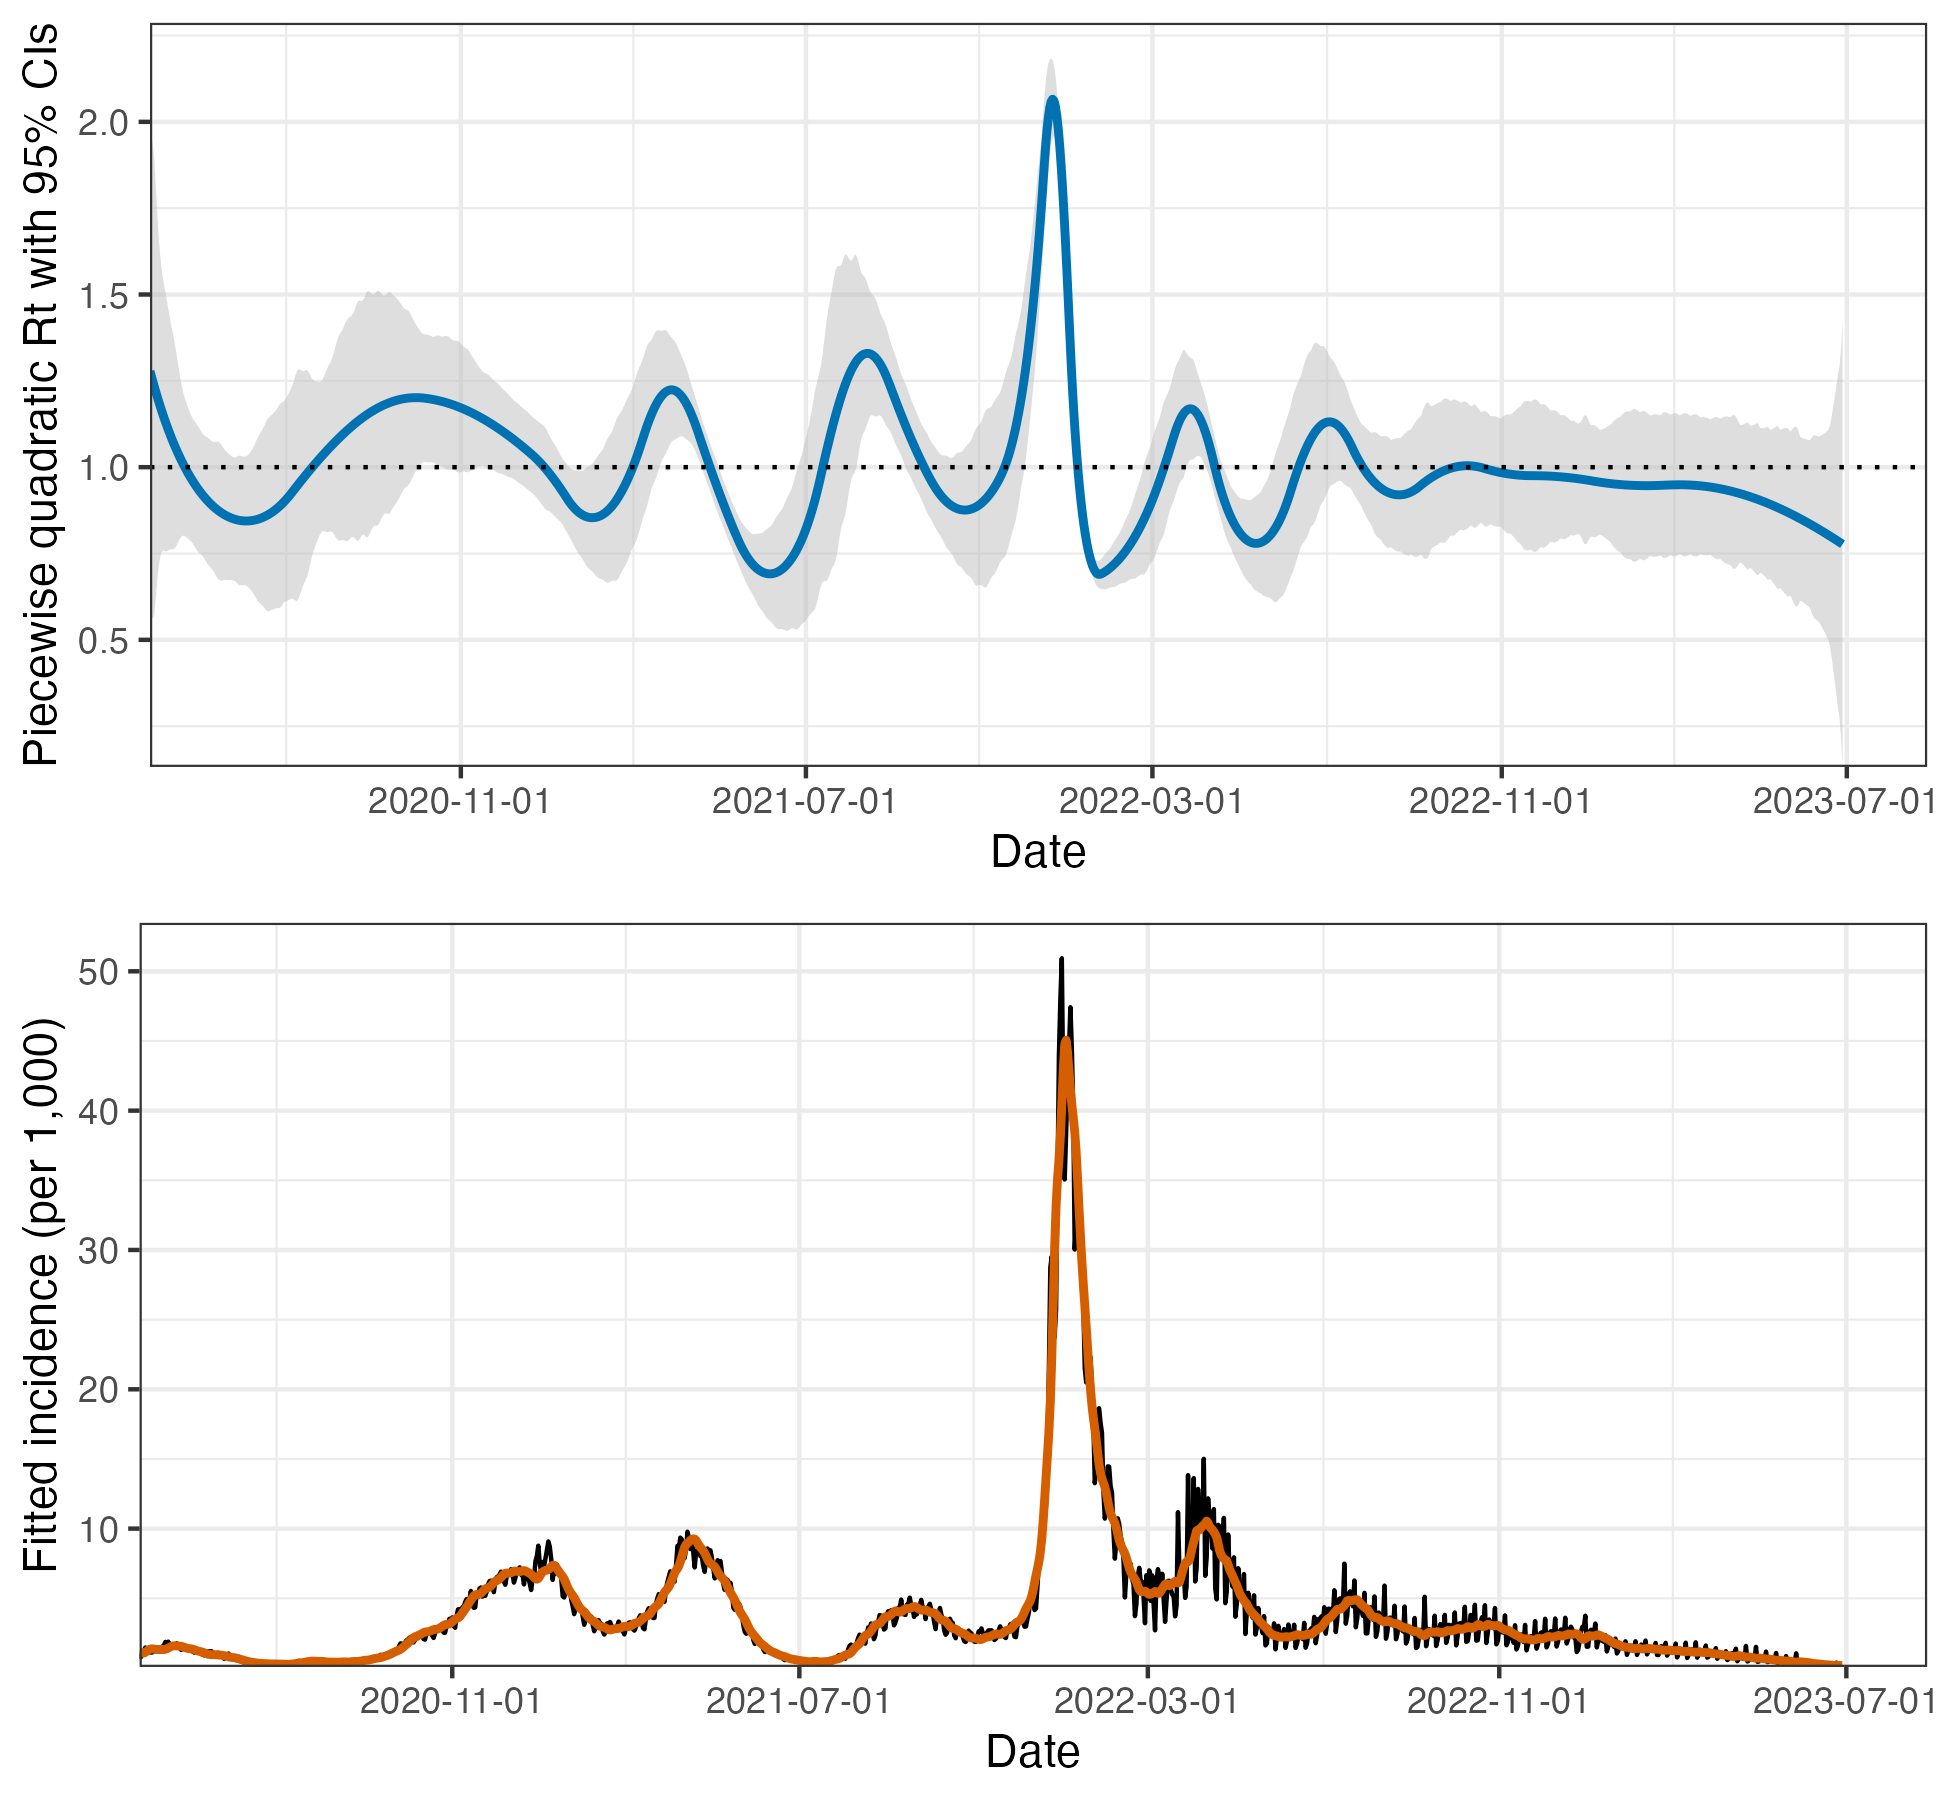
\includegraphics[width=.9\textwidth]{fig/intro-fig-new.png}
  \caption{A demonstration of effective reproduction number estimation 
  by \RtEstim\ and the corresponding predicted incident cases for the Covid-19 
  epidemic in Canada during the period from January 23, 2020 to June 28, 2023. 
  In the top panel, the blue curve is the estimated piecewise quadratic $\calR_t$ 
  and the colorful ribbon is the corresponding 95\% confidence band. 
  The ribbon is dyed by four colors representing the variants whose serial interval 
  distributions are used to estimate $\calR_t$. The y-axis is truncated for 
  a better illustration; the estimated $\calR_t$ decreases from $10.77$ to below $2$
  in the first 55 timepoints. In the bottom panel, the black curve is the observed Covid-19 
  daily confirmed cases, and the orange curve on top of it is the predicted incident cases
  corresponding to the estimated $\calR_t$. The three vertical dashed lines 
  represent the beginning of a new dominant variant.}
  \label{fig:intro-fig}
\end{figure}

While our approach is straightforward and requires little domain knowledge for
implementation, we also implement a number of refinements. 
We use a proximal Newton method to solve the convex optimization problem along
with warm starts to produce estimates efficiently, typically in a matter of 
seconds, even for long sequences of data. In a number of simulation experiments, 
we show empirically that our approach is more \textit{accurate} than existing methods at 
estimating the true effective reproduction numbers and \textit{robust} under multiple 
settings of the misspecification of incidence distribution, serial interval 
distribution, and the order of graphical curvature. 


The manuscript proceeds as follows. We first introduce the methodology of
\RtEstim\ including the renewal equation and the development of Poisson
trend filtering estimator. We explain how this method could be interpreted from
the Bayesian perspective, connecting it to previous work in this context. We
provide illustrative experiments comparing our estimator to other Bayesian alternatives. 
We then apply our \RtEstim\ on the Covid-19 pandemic in Canada and 
the 1918 influenza pandemic in the United States. Finally, we conclude 
with a discussion of the advantages and limitations of our approach and describe 
practical considerations for effective reproduction number estimation.


\section{Methods}

\subsection{Renewal model for incidence data} 

The effective reproduction number $\calR(t)$ is defined to be the expected
number of secondary infections at time $t$ produced by a primary infection
sometime in the past. To make this precise, denote the number of new infections
at time $t$ as $y(t)$. Then the total primary infectiousness can be written as
$\eta(t) := \int_0^{\infty} p(t,i) y(t-i) \diff i$, where $p(t,i)$ is the
probability that a new secondary infection at time $t$ is the result of a primary infection
that occurred $i$ time units in the past. The effective reproduction number is then given
as the value that equates
\begin{equation} \label{eq:pre-renew-equation}
  \bbE[y(t) \mid y(j),\ j<t]=\calR(t)\eta(t)=\calR(t)\int_0^\infty p(t,i)y(t-i)\diff i,
\end{equation}
otherwise known as the renewal equation. The period between primary and secondary
infections is exactly the generation time of the disease, but given real data,
observed at discrete times (say, daily), this delay distribution must be discretized
into contiguous time intervals,
say, $(0,1], (1,2], \cdots$. It results in the sequence $\{p^t_i\}_{i=0}^\infty$
corresponding to observations $y_t$ for each $t$ and yields the
discretized version of \eqref{eq:pre-renew-equation},
\begin{equation} \label{eq:renew-equation}
  \bbE[y_t \mid y_1,\ldots,y_{t-1}]=\calR_t\eta_t=\calR_t\sum_{i = 1}^\infty p^t_i y_{t-i}.
\end{equation}
Many approaches to estimating $\calR_t$ rely on \eqref{eq:renew-equation} as
motivation for their procedures, among them, \EpiEstim\ \citep{cori2013new} 
and \texttt{EpiFilter} \citep{parag2021improved}. 


In most cases, it is safe to assume that infectiousness disappears beyond 
$\tau$ timepoints ($p(t,i) = 0$ for $i > \tau$), resulting in the truncated integral 
of the generation interval distribution $\int_0^\tau p(t,i)\diff i = 1$ for each $t$.
Generation time, however, is usually unobservable and tricky to estimate, so
common practice is to approximate it by the serial interval: the period between
the symptom onsets of primary and secondary infections. If the infectiousness
profile after symptom onset is independent of the incubation period (the period
from the time of infection to the time of symptom onset), then this
approximation is justifiable: the serial interval distribution and the
generation interval distribution share the same mean. However, other properties
may not be similarly shared, and, in general, the generation interval
distribution is a convolution of the serial interval distribution with the
distribution of the difference between independent draws from the delay
distribution from infection to symptom onset. See, for example,
\cite{gostic2020practical} for a fuller discussion of the dangers of this
approximation. Nonetheless, treating these as interchangeable is common
\citep{cori2013new,park2021forward} and doing otherwise is beyond the scope of this work. 
Additionally, we take the generation interval (and, therefore, the 
serial interval) either as constant over time $t$, i.e., the probability $p(i)$ 
depends only on the gap between primary and secondary infections and not on 
the time $t$ when the secondary infection occurs, or as time-varying, i.e., 
the probability $p(t,i)$ also depends on the time of (the symptom onset of)
the secondary infection. For our methods, we 
assume that the serial interval can be accurately estimated from auxiliary 
data (say by contact tracing, or previous epidemics) and we take it as 
fixed, as is common in existing studies, e.g., 
\cite{cori2013new,abry2020spatial,pascal2022nonsmooth}.


The renewal equation in \eqref{eq:renew-equation} relates observable data
streams (incident cases) occurring at different timepoints to the effective reproduction
number given the serial interval. The fact that it depends only on the observed
incident counts makes it reasonable to estimate $\calR_t$. However, 
data collection idiosyncrasies can obscure this relationship. Diagnostic testing
targets symptomatic individuals, omitting asymptomatic primary infections which
can lead to future secondary infections. Testing practices, availability, and
uptake can vary across space and time \citep{pitzer2021impact,
hitchings2021usefulness}. Finally, incident cases as reported to public health
are subject to delays due to laboratory confirmation, test turnaround times, and
eventual submission to public health \citep{pellis2021challenges}. For these
reasons, reported cases are lagging indicators of the course of the pandemic.
Furthermore, they do not represent the actual number of new infections that
occur on a given day, as indicated by exposure to the pathogen. The assumptions
described above (homogeneous mixing,
similar susceptibility and social behaviours, etc.) are therefore consequential.
That said, \eqref{eq:renew-equation} also provides some comfort about deviations
from these assumptions. Under certain conditions, failing to account for the 
reporting delay will minimally impact the accuracy of any $\mathcal{R}_t$ estimator 
that is based on \eqref{eq:renew-equation}. We discuss three types of deviation here.
First, if $y_t$ is scaled by a constant (in time) describing
the reporting ratio, then it will cancel from both sides when we take the ratio
of secondary and primary infection when calculating the effective reproduction 
number. Second, even if such a scaling varies in time, as long as it varies slowly relative
to the set of $p_i$ that are larger than 0, \eqref{eq:renew-equation} will be a
reasonably accurate approximation, so that $\calR_t$ can still be estimated well
from reported incidence data. Finally, even a sudden change in reporting ratio
occurs at time $t_1$, it would only result in 
large errors in $\calR_t$ in the neighbourhood of $t_1$ (where the size of this 
neighbourhood is determined indirectly by the effective support of $\{p^t_i\}$). 
This robustness to certain types of data reporting issues partially justifies 
using \eqref{eq:renew-equation} to calculate $\calR_t$.


\subsection{Poisson trend filtering estimator} 

We use the daily confirmed incident cases $y_t$ on day $t$ to estimate the
observed infectious cases under the model that $y_t$, given previous incident
cases $y_{t-1},\ldots,y_1$ and a constant serial interval distribution, follows a
Poisson distribution with mean $\Lambda_t$. That is, 
\begin{equation}
  y_t \mid y_1,\ldots,y_{t-1} \sim \mathrm{Poisson}(\Lambda_t), \textrm{ where } 
  \Lambda_t =  \calR_t\sum_{i=1}^{t-1}p_i y_{t-i} = \calR_t\eta_t.
\end{equation} 
Given a history of $n$ confirmed incident counts $\bfy = {(y_1,\ldots,y_n)}^\top$,
our goal is to estimate $\calR_t$ for each $t=1,\cdots,n$. A natural approach is to maximize the
likelihood, producing the maximum likelihood estimator (MLE):
\begin{equation} \label{eq:mle}
  \begin{split}
    \widehat{\calR} &= \Argmax{\calR \in \bbR_+^n} \bbP(\calR \mid \bfy,\ \bfp)
    = \Argmax{\calR \in \bbR^n_+} \prod_{t = 1,\dots,n} 
    \frac{\lr{\calR_t \eta_t}^{y_t} \exp\{- \calR_t \eta_t\}  }{y_t!}\\
    &= \Argmin{\calR\in\bbR^n_+} \sum_{t = 1}^n \calR_t\eta_t - 
    y_t\log(\calR_t\eta_t).
  \end{split}
\end{equation}
This optimization problem, however, is easily seen to yield a one-to-one
correspondence between the observation and the estimated effective reproduction
number, i.e.,
$\widehat{\calR}_t = y_t / \eta_t$, so that the estimated sequence
$\widehat{\calR}$ will have no significant smoothness.


The MLE is an unbiased estimator of the true parameter $\calR_t$, but
unfortunately has high variance: changes in $y_t$ result in proportional changes
in $\widehat\calR_t$. To avoid this behaviour, and to match the intuition that
$\calR_t \approx \calR_{t-1}$, we advocate enforcing smoothness of the effective
reproduction numbers. This constraint will decrease the estimation variance, and
hopefully lead to more accurate estimation of $\calR$, as long as the smoothness
assumption is reasonable. Smoothness assumptions are common (see e.g.,
\cite{gostic2020practical,parag2021improved}), but the type of
smoothness assumption is critical. Cori et al. imposes smoothness
indirectly by estimating $\calR_t$ with moving windows of past observations \citep{cori2013new}. The
Kalman filter procedure of \cite{parag2021improved} would enforce in 
$\ell_2$-smoothness ($\int_0^n {(\widehat{\calR}''(t))}^{2}\diff t < C$ for some 
constant $C$), although the computational implementation results in $\widehat{\calR}$
taking values over a discrete grid. Pascal et al. produces
piecewise linear $\widehat{\calR}_t$, which turns out to be closely related to a
special case of our methodology \citep{pascal2022nonsmooth}. Smoother estimated curves will provide
high-level information about the entire epidemic, obscuring small local changes
in $\calR(t)$, but may also remove the ability to detect large sudden changes,
such as those resulting from lockdowns or other major containment policies. 

To enforce smoothness of $\hat\calR_t$, we add a trend filtering penalty to
\eqref{eq:rt-ptf} \citep{kim2009ell_1, tibshirani2014adaptive, tibshirani2022divided, 
sadhanala2024exponential}. Because $\calR_t > 0$,
we explicitly penalize the divided differences (discrete derivatives) of
neighbouring values of $\log(\calR_t)$. 
Let $\theta := \log(\calR) \in \bbR^n$, so that $\Lambda_t =
\eta_t \exp(\theta_t)$, and $\log(\eta_t \calR_t) = \log(\eta_t) +
\theta_t$. For evenly spaced incident case, we
write our estimator as the solution to the optimization problem
\begin{equation} 
  \label{eq:rt-ptf}
  \widehat{\calR} = \exp(\widehat{\theta}) \quad\textrm{where}\quad \widehat{\theta} 
  = \Argmin{\theta\in\bbR^n} \eta^\top \exp(\theta) - \bfy^\top \theta + \lambda 
  \snorm{D^{(k+1)} \theta}_1,
\end{equation}
where $\exp(\cdot)$ applies elementwise and $\snorm{\boldsymbol{a}}_1 := \sum_{i=1}^n |a_i|$ is the $\ell_1$ norm.
Here, $D^{(k+1)} \in \bbZ^{(n-k-1)\times n}$ is the $(k+1)\th$ order divided
difference matrix for any $k \in \{0,\ldots,n-1\}$. 
$D^{(1)} \in \{-1,0,1\}^{(n-1)\times n}$ is the divided difference matrix for $k=0$. 
It is a sparse matrix with diagonal band of the form:
\begin{equation} 
  \label{eq:d1mat}
  D^{(1)} = 
  \begin{pmatrix} 
    -1 & 1 &  & & \\ 
    & -1 & 1 & & \\ 
    & & \ddots & \ddots & \\
    & & & -1 & 1 
  \end{pmatrix}.
\end{equation}
$D^{(k+1)}$ for $k\geq 1$ is defined recursively as $D^{(k+1)} := D^{(1)} D^{(k)}$, where 
$D^{(1)} \in \{-1,0,1\}^{(n-k-1)\times (n-k)}$ takes the form defined in \eqref{eq:d1mat}. 
More description on the recursive definition of divided difference matrix for trend filtering
can be found in \cite{tibshirani2014adaptive,tibshirani2022divided}.

The tuning parameter (hyperparameter) $\lambda$ balances data
fidelity with desired smoothness. When $\lambda=0$, the problem in
\eqref{eq:rt-ptf} reduces to the MLE in \eqref{eq:mle}. Larger tuning parameters
privilege the regularization term and yield smoother estimates. Finally, there
exists $\lambda_{\textrm{max}}$ such that any $\lambda \geq
\lambda_{\textrm{max}}$ will result in $D^{(k+1)} \widehat {\theta} = 0$ and
$\widehat{\theta}$ will be the Kullback-Leibler projection of $\bfy$ onto the
null space of $D^{(k+1)}$ (see \autoref{sec:candidate-set}).

The solution to \eqref{eq:rt-ptf} will result in piecewise
polynomials, specifically called discrete splines. For example, $0\th$-degree
discrete splines are piecewise constant, \first-degree curves are piecewise
linear, and \second-degree curves are piecewise quadratic. For $k\geq 1$,
$k\th$-degree discrete splines are continuous and have continuous discrete
differences up to degree $k-1$ at the knots (i.e., changing points between segments). This penalty results in more
flexibility compared to the homogeneous smoothness that is created by the
squared $\ell_2$ norm. Using different orders of the divided differences results in
estimated effective reproduction numbers with different smoothness properties. 



For unevenly spaced data, the spacing between neighbouring parameters
varies with the time between observations, and thus, the divided differences
must be adjusted by the times that the observations occur. Given observation
times $\bfx = {(x_1,\dots,x_n)}^\top$, for $k \geq 1$, define a $k\th$-order
diagonal matrix 
\begin{equation}
  X^{(k)} = \diag \lr{\frac{k}{x_{k+1} - x_1},\ \frac{k}{x_{k+2} - x_2},\ 
  \cdots,\ \frac{k}{x_n - x_{n-k}} }.
\end{equation}
Letting $D^{(\bfx,1)} := D^{(1)}$,
then for $k\geq 1$, the $(k+1)\th$-order divided difference matrix for unevenly
spaced data can be created recursively by
$D^{(\bfx, k+1)} := D^{(1)} X^{(k)} D^{(\bfx,k)}.$ No adjustment is required
for $k=0$. 


Due to the penalty structure, this estimator is locally adaptive,
meaning that it can potentially capture local changes such as the initiation of
control measures. Abry et al. and Pascal et al. considered only the
\second-order divided difference of $\calR_t$ rather than its logarithm 
\citep{abry2020spatial,pascal2022nonsmooth}. In
comparison to their work, our estimator (i) allows for arbitrary degrees of
temporal smoothness and (ii) avoids the potential numerical issues of
penalizing/estimating positive real values. Furthermore, as we will describe
below, our procedure is computationally efficient for estimation over an entire
sequence of penalty strengths $\lambda$ and provides methods for choosing how
smooth the final estimate should be.


\subsection{Solving over a sequence of tuning parameters}
\label{sec:candidate-set}

We can solve the Poisson trend filtering estimator over an arbitrary sequence of 
$\lambda$ that produces different levels of smoothness in the estimated curves. 
We consider a candidate set of M $\lambda$-values, $\boldsymbol{\lambda} = \{\lambda_m\}_{m=1}^M$,
that is strictly decreasing.


Let $D := D^{(k+1)}$ for simplicity in the remainder of this section. As
$\lambda \to\infty$, the penalty term $\lambda \snorm{D\theta}_1$ dominates the
Poisson objective, so that minimizing the objective is asymptotically equivalent
to minimizing the penalty term, which results in $\snorm{D\theta}_1 = 0$. In
this case, the divided differences of $\theta$ with order $k+1$ is always $0$,
and thus, $\theta$ must lie in the null space of $D$, that is,
$\theta\in\mathcal{N}(D)$. The same happens for any $\lambda$ beyond this
threshold, so define $\lambda_{\textrm{max}}$ to be the smallest $\lambda$ that
produces $\theta\in\mathcal{N}(D)$. It turns out that this value can be written
explicitly as $\lambda_{\textrm{max}} = \snorm{\lr{D^{\dagger}}^{\top} \lr{\eta
- y}}_{\infty},$ where $D^{\dagger}$ is the (left) generalized inverse of $D$
satisfying $D^{\dagger} D = I$ and $\snorm{a}_{\infty} := \mathrm{max}_{i=1}^n\{|a_i|\}$ is the infinity norm. 
Therefore, we use $\lambda_1 =
\lambda_{\textrm{max}}$ and then choose the minimum $\lambda_M$ to be
$r\lambda_{max}$ for some $r \in (0,1)$ (typically $r=10^{-5}$). Given any
$M\geq 3$, we generate a sequence of $\lambda$ values to be equally spaced on
the log-scale between $\lambda_1$ and $\lambda_M$. 

To compute the sequence efficiently, the model is estimated sequentially by
visiting each component of $\boldsymbol{\lambda}$ in order. The estimates
produced for a larger $\lambda$ are used as the initial values (warm starts) for
the next smaller $\lambda$. By solving through the entire sequence of tuning
parameters, we have a better chance to achieve a better trade-off between bias
and variance, and accordingly, improved accuracy relative to procedures
examining one fixed value of $\lambda$.


\subsection{Choosing a final $\lambda$}
\label{sec:cv}

We estimate model accuracy over the candidate set through $K$-fold cross
validation (CV) to choose the best tuning parameter. Specifically, we divide
$\bfy$ (except the first and last observations) roughly evenly and randomly into
$K$ folds, estimate $\calR_t$ for all $\boldsymbol{\lambda}$ leaving one fold
out, and then predict the held-out observations. 
An alternative splitting of observations is regular splitting, where we assign every
$k\th$ observation into the same fold. Note that our approach is most closely
related to non-parametric regression rather than time series forecasting. That
said, under some conditions, one can guarantee that $K$-fold is valid for risk
estimation in time series. The sufficient conditions are quite strong, but the
guarantees are also stronger than would be required for model selection
consistency \citep{BERGMEIR201870}. 

Model accuracy can be measured
by multiple metrics such as mean squared error $\mathrm{MSE}(\widehat{y},\ y) =
n^{-1}\snorm{\widehat{y} - y}_2^2$ or mean absolute error
$\mathrm{MAE}(\widehat{y},\ y) = n^{-1}\snorm{\widehat{y} - y}_1$, but we prefer
to use the (average) deviance, to mimic the likelihood in \eqref{eq:mle}:
$D\lr{y,\ \hat{y}} = n^{-1}\sum_{i=1}^n 2\lr{y_i \log(y_i) - y_i\log(\hat{y}_i)
- y_i + \hat{y}_i},$ with the convention that $0\log(0) = 0$. Note that for any $K$ and any $M$, we will end up 
estimating the model $(K+1)M$ times rather than once.


\subsection{Approximate confidence bands} 
\label{sec:conf-band} 

We also provide empirical confidence bands of the estimators with  
approximate coverage. Consider the related estimator $\widetilde{\calR}_t$
defined as
\begin{equation}
  \widetilde{\calR} = \exp(\widetilde{\theta}) \quad\textrm{where}\quad
  \widetilde{\theta} = \Argmin{\theta\in\bbR^n} \eta^\top \exp(\theta) - \bfy^\top
  \theta + \lambda \snorm{D \theta}_2^2.
\end{equation}
Let $\widetilde{\bfy} = \eta \circ \widetilde\calR$, and then it can be shown (for example,
Theorem 2 in \cite{vaiter2017degrees}) that an estimator for
$\Var(\widetilde{\bfy})$ is given by $\big(\mathrm{diag}(\widetilde{\bfy}^{-2})
+ \lambda D^{\top} D\big)^{\dagger}.$ Finally, an
application of the delta method shows that $\Var(\widetilde{\bfy}_t) / \eta_t^2$
is an estimator for $\Var(\widetilde{\calR}_t)$ for each $t = 1, \ldots, n$. We
therefore use ${\big(\mathrm{diag}(\widehat{\bfy}^{-2}) + \lambda
D^{\top} D\big)}^{\dagger}_t / \eta_t^2$ as an estimator
for $\Var(\widehat{\calR}_t)$. An approximate $(1-\alpha)\%$ confidence interval
then can be written as $\widehat{\calR}_t\pm s_t \times T_{\alpha/2,n-\textrm{df}}$, 
where $s_t$ is the square-root of $\Var(\widehat{\calR}_t)$ for each 
$t = 1, \cdots, n$ and $\textrm{df}$ is the number of changepoints in 
$\widehat{\theta}$ plus $k+1$ \citep{tibshirani2014adaptive}. 
An approximate confidence interval of $\hat{\bfy}$ can be computed similarly. 


\subsection{Bayesian perspective}

Unlike many other methods for $\calR_t$ estimation, our approach is frequentist
rather than Bayesian. Nonetheless, it has a corresponding Bayesian
interpretation: as a state-space model with Poisson observational noise,
autoregressive transition equation of degree $k\geq 0$, e.g., $\theta_{t+1} =
2\theta_t - \theta_{t-1} + \varepsilon_{t+1}$ for $k=1$, and Laplace transition
noise $\varepsilon_{t+1}\sim \mathrm{Laplace}(0,\ 1/\lambda)$. Compared to
\texttt{EpiFilter} \citep{parag2021improved},
 we share the same observational assumptions, but our approach has a
different transition noise. \texttt{EpiFilter} estimates the posterior
distribution of
$\calR_t$, and thus it can provide credible interval estimates as well. Our
approach produces the maximum \emph{a posteriori} estimate via an efficient
convex optimization, obviating the need for MCMC sampling. But the associated
confidence bands are created differently.


\section{Results}

Implementation of our approach is provided in the \R\ package
\href{https://dajmcdon.github.io/rtestim/}{\texttt{rtestim}}. 
All computational experiments are conducted on the Cedar cluster provided 
by Compute Canada with \texttt{R 4.3.1}. The \R\ packages used for
simulation and real-data application are \texttt{EpiEstim 2.2-4} \citep{Cori2022},
\texttt{EpiLPS 1.2.0} \citep{Gressani2021}, and \texttt{rtestim 0.0.4}. 
The \R\ scripts for \EpiFilter\ are used \citep{kpzoo2020}.

\subsection{Synthetic experiments}

\subsubsection{Problem design}

We simulate four scenarios of the time-varying effective reproduction number,
intended to mimic different epidemics. The first two scenarios are rapidly 
controlled by intervention, where the $\calR(t)$ consists
of one discontinuity and two segments. Scenario 1 has constant $\calR(t)$ before
and after an intervention, while Scenario 2 grows exponentially, then decays.
The other two scenarios are more complicated, where more waves
are involved. Scenario 3 has four linear segments with three discontinuities,
which reflect the effect of an intervention, resurgence to rapid transmission,
and finally suppression of the epidemic. Scenario 4 involves sinusoidal waves
throughout the epidemic.
The first three scenarios and the last scenario are motivated by
\cite{parag2021improved} and \cite{gressani2022epilps} respectively. 
We name the four scenarios as \textit{(1) piecewise constant}, \textit{(2) 
piecewise exponential}, \textit{(3) piecewise linear}, and \textit{(4) periodic} 
lines or curves respectively. 

In all cases, the times of observation are regular, and epidemics are of
length $n=300$. Specifically, in Scenario 1, $\calR_t = 2, 0.8$ before and after
$t=120$. In Scenario 2, $\calR_t$ increases and decreases exponentially with
rates $0.01, 0.005$ pre and post $t=100$. 
In Scenario 3, $\calR_t$ is piecewise linear with four discontinuous segments following 
\begin{equation}
  \begin{split}
    \calR(t) =& \lr{2.5 - \frac{0.5}{74}\lr{t-1}} \boldsymbol{1}_{[1,76)}(t)
     + \lr{0.8 - \frac{0.2}{74}\lr{t-76}} \boldsymbol{1}_{[76,151)}(t) \\
    & + \lr{1.7 + \frac{0.3}{74}\lr{t-151}} \boldsymbol{1}_{[151,226)}(t)
       + \lr{0.9 - \frac{0.4}{74}\lr{t-226}} \boldsymbol{1}_{[226,300]}(t),
  \end{split}
\end{equation}
where $\boldsymbol{1}_{A}(t) = 1$, if $t\in A$, and $\boldsymbol{1}_{A}(t)=0$ otherwise. 
In Scenario 4, $\calR_t$ is realization of the 
continuous, periodic curve generated by the function 
\begin{equation}
  \calR(t) = 0.2 \big(\lr{\sin(\pi t/12) + 1} + \lr{2 \sin\lr{5 \pi t / 12} + 2} 
  + \lr{3 \sin(5\pi t / 6) + 3}\big),
\end{equation} 
evaluated at equally spaced points $t\in [0,10]$. 
These $\calR_t$ scenarios are illustrated in \autoref{fig:samples}.
We compute the expected incidence $\Lambda_t$
using the renewal equation, and generate the incident infections from the
Poisson distribution $y_t\sim \textrm{Pois}(\Lambda_t)$. 
To verify the performance of our model under the violation of the distributional assumption,
we also generate incident cases using the negative binomial distribution
with dispersion size $\rho=5$, i.e., $y_t\sim \textrm{NB}(\mu_t=\Lambda_t,
\rho=5)$. The probability mass function can be written as 
\begin{equation}
  \begin{split}
    p(y_t|\Lambda_t,\rho) = \frac{\Gamma(y_t+\rho)}{\Gamma(\rho)y_t!} \Big(\frac{\rho}{\rho+\Lambda_t}\Big)^{\rho} \Big(\frac{\Lambda_t}{\rho+\Lambda_t}\Big)^{y_t},  
  \end{split}
\end{equation}
where $y_t = 0,1,2,\cdots, t=1,\cdots,n$ and the variance is
 $\sigma_t^2 = \Lambda_t + \frac{\Lambda_t^2}{\rho}$, which follows the 
 definition in \cite{gressani2022epilps}.
The variance equals the mean appended by another term of the squared mean over a
relatively small dispersion size, so the squared mean can dominate the term and
result in sufficient overdispersion level in the generated samples. 
We visualize the dispersion level (using the ratio of standard deviation over mean) 
of synthetic epidemics in Figure A.2.1 in the supplementary document to have a better idea on the overdispersion level 
of the negative binomial distributions (with size 5) compared the Poisson 
distributions with the same mean. 

We use serial interval (SI) distributions of measles (with mean $14.9$ and standard 
deviation $3.9$) at Hagelloch, Germany in 1861 \citep{groendyke2011bayesian} and 
SARS (with mean $8.4$ and standard deviation $3.8$) at Hong Kong in 2003 
\citep{lipsitch2003transmission}, inspired by \cite{cori2013new}, to generate synthetic 
epidemics. We initialize all epidemics with $y_1=2$ cases and generate for $t=2,\ldots,300$. 
The synthetic measles epidemics have smaller incident cases in general, and the SARS 
epidemics have larger incidence. The intuition behind this is a smaller mean
of serial interval with a similar standard deviation leads to an averaged shorter period 
of the onsets of symptoms between the primary and secondary infected individuals, which 
results in a greater growth of incidence within the same period of time. 
We also consider shorter flu epidemics with 50 timepoints with piecewise linear $\calR_t$ (Scenario 3)
considering both incidence distributional assumptions. The motivation is to compare our method and 
other alternatives with EpiNow2 which takes much longer time to converge 
for long epidemics (almost 2 hours to converge for a measles epidemic 
with 300 timepoints) than other methods.  
Besides using the correct SI distributions to estimate $\calR_t$, we also consider 
the scenarios where SI is mildly or majorly misspecified. 
More details on experimental settings and results for shorter epidemics and misspecification 
of SI distributions are given in Sections A.2.1 and A.3 in the supplementary document respectively. 

For each problem setting (including a SI distribution, an $\calR_t$ scenario, 
and an incidence distribution), we generate 50 random samples, resulting in 
$800$ total synthetic epidemics. 
An example of measles and SARS epidemics for each effective reproduction number scenario
with an incidence distribution is displayed in \autoref{fig:samples}. 

\begin{figure}[!ht]
  \centering
  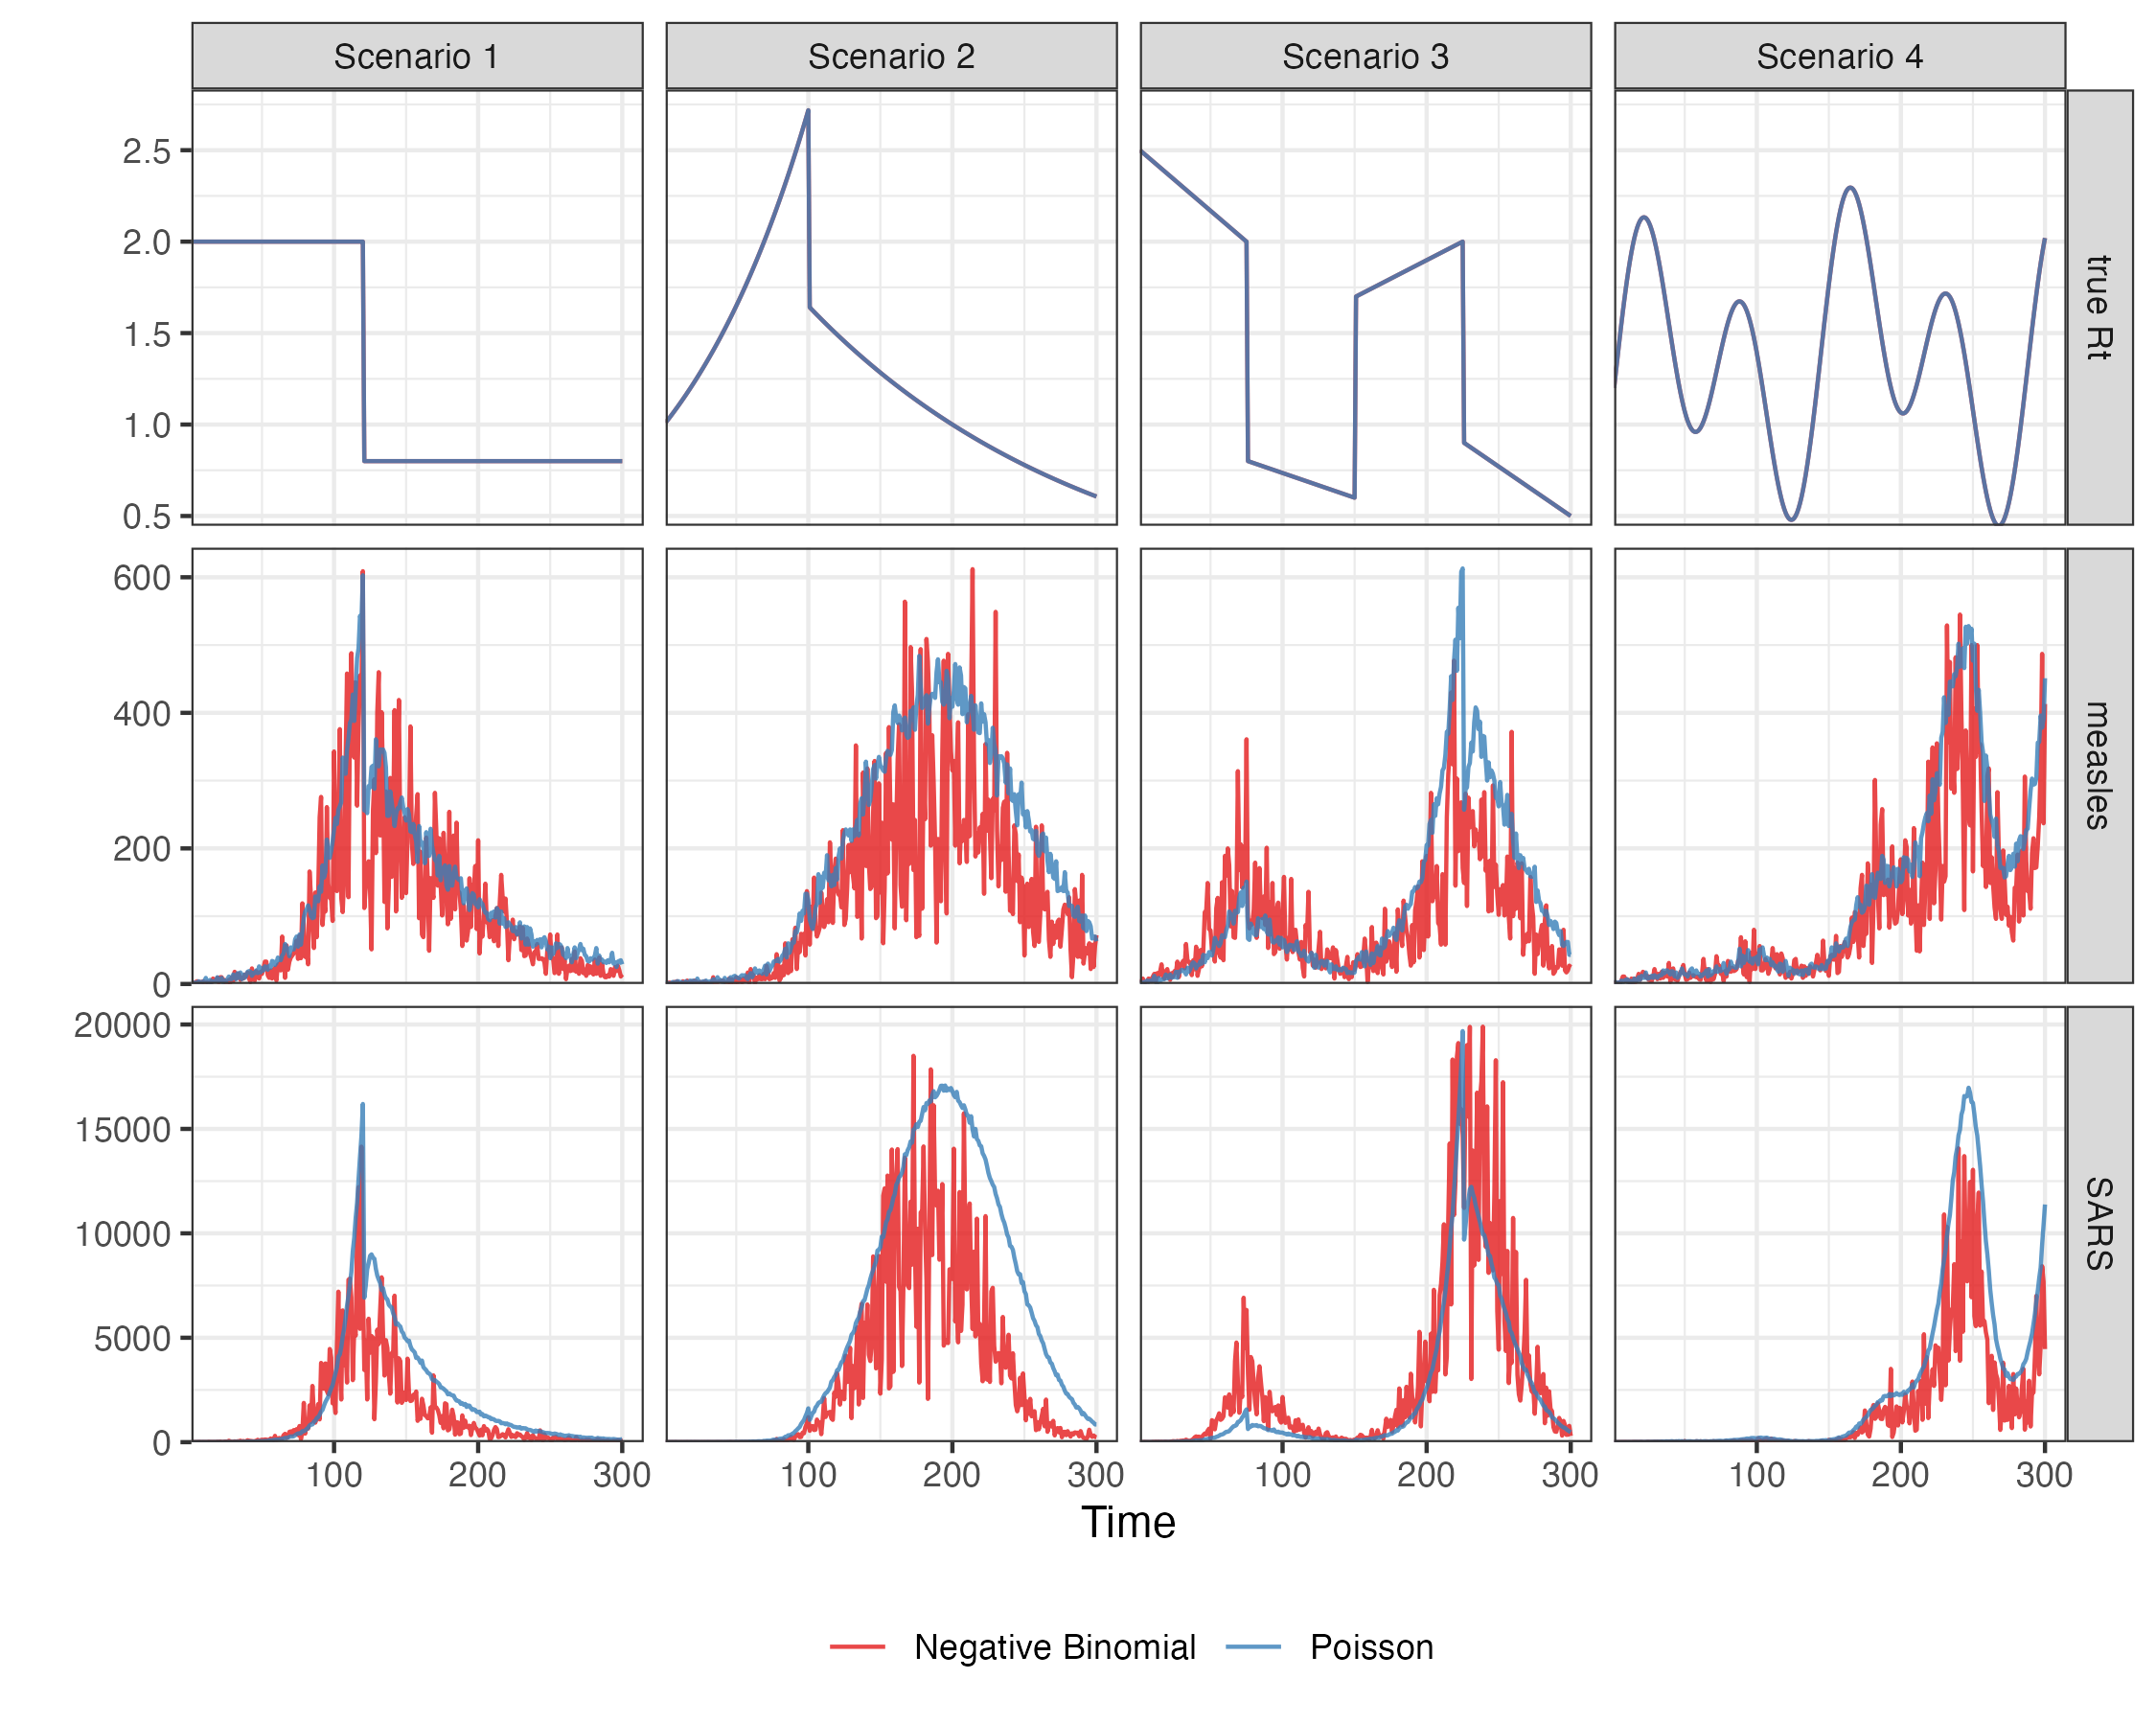
\includegraphics[width=1.0\textwidth]{fig/fig_samples.png}
  \caption{The \textbf{effective reproduction numbers} for four $\calR_t$ scenarios (\textit{in the top row}). 
  The synthetic measles (\textit{in the middle row}) and SARS (\textit{in the bottom row}) \textbf{incident cases} drawn 
  from Poisson (\textit{in blue curves}) or negative binomial (\textit{in red curves}) distribution 
  across 4 $\calR_t$ scenarios (\textit{in four columns respectively}).} 
  \label{fig:samples}
\end{figure}

\subsubsection{Algorithm design}

We compare \RtEstim\ to \EpiEstim, \EpiLPS, and \EpiFilter. \EpiEstim\ estimates
the posterior distribution of the effective reproduction number given a Gamma
prior and Poisson distributed observations
over a trailing window, under the assumption that the effective reproduction number is
constant during that window. A larger window averages out more fluctuations,
leading to smoother estimates, whereas, a shorter sliding window is more
responsive to sudden spikes or declines. We tried the weekly sliding
window, as well as a monthly window. However, since neither considerably
outperforms the other across all scenarios, we defer the monthly results to the
supplementary document. \EpiLPS\ is another Bayesian approach that estimates P-splines 
based on the Laplace approximation to the conditional posterior with negative
binomial likelihood. \texttt{EpiFilter} is also a Bayesian approach that smooths 
$\calR_t$ at each timepoint given all observed incidence, improved upon the filtering methods
that filter $\calR_t$ given the observations prior to and on time $t$.

We apply \RtEstim\ with four degrees, piecewise constant $k=0$, piecewise linear $k=1$, 
piecewise quadratic $k=2$, and piecewise cubic $k=3$ polynomials, to solve all problem settings.
We run 10-fold cross validation (CV) to choose the best tuning parameter
from the candidate set of size $50$, i.e., $\boldsymbol{\lambda} = \{\lambda_1,
\cdots, \lambda_{50}\}$, for long epidemics, and $5$-fold CV for short epidemics 
(deferred to Sections A.3.2 and A.4.2 in the supplementary document). 
Specifically, we divide all samples (except the first and last entries) into
$10$ folds evenly and randomly, and build models on each subset of samples 
by leaving a fold out using each choice of the tuning parameter. We select the 
tuning parameter that gives the lowest averaged deviance between the 
estimated incidence and the observed samples averaged over all folds. 

We specify the parameters of the alternative methods, using the ones which were 
applied to their own experimental settings and so are deemed as the ``best'' tuned 
ones, in our experiments. Due to the limitations of the software implementations that
some necessary hyperparameters are not allowed to choose, we can only specify 
the supported ones. 
This limitation does not only restrict the choices on tuning parameters which impacts 
the model fitting, but also those for optimization (as mentioned above). 
For example, in EpiLPS, one must specify the number of basis functions as well as 
$5$ prior parameters. EpiFilter needs a grid of possible $\calR_t$ values, 
along with the a fixed value for the diffusion noise, and a prior value for 
$\calR_t$. \EpiNow2\ has many prior parameters (depending on the particular model 
used) and does not compute a Bayes Factor or other model selection criterion. 
Had we attempted to tune some or all of these parameters, we would need to 
implement cross validation from scratch for each, as none of these provide 
ways to choose them. 
Here are the hyperparameters used in modelling for each alternative method. 
We consider both weekly and monthly sliding windows in \EpiEstim, 
40 basis functions in \EpiLPS\ with the NelderMead method to maximize the 
hyperparameter posterior distribution. We input 2000 grid size in \EpiFilter\ 
with 0.1 diffusion noise and uniform prior on $\calR_t$ with mean 
1/2000, and use the smoothed $\calR_t$ given all observed incidence as the final 
estimates. 

For the $\calR_t$ estimation using all models for each problem, we use the same serial 
interval distribution, that was used to generate synthetic data. Taking different 
hyperparameters into consideration, we solve each problem using 8 methods including 
\EpiEstim\ with weekly or monthly sliding windows, \EpiLPS, \EpiFilter, and 
\RtEstim\ with piecewise constant, linear, quadratic, or cubic curves. 
% discuss `degree' of all methods
Throughout the four $\calR_t$ scenarios, the degrees of \RtEstim\ can be correctly or 
wrongly specified. Our method can take the advantage of a correctly specified 
degree of piecewise polynomials compared to other methods, while the competitors only 
consider one fixed degree of smoothness which may not coincide with the ``true'' 
(assumed) degree of $\calR_t$.
Meanwhile, by using different degrees to solve the same problem, we will illustrate 
that a wrongly specified degree can still result in accurate $\calR_t$ estimation 
in our experiments. 

\RtEstim\ estimates can appear to be piecewise polynomials with a selected degree 
$k$. % where the changing points of polynomial segments are completely data driven. 
When faced with real data, the choice of $k$ should be done either (1)
based on the analyst's preference for the result (e.g., ``I want to find
large jumps, so $k=0$'') or (2) in a data-driven manner, as a component of the
estimation process. Our software enables both cases, and the second case can be 
implemented by simply fitting for different $k$ and choosing the set $k,\lambda$ 
that has smallest CV score. Thus, all necessary choices can be accomplished based 
solely on the data. Our software is a departure from existing methods in that 
we \emph{allow} this choice and provide simple data-driven methods to accomplish it. 
\EpiEstim\ has no such facility (although, implicitly, one must somehow choose the 
size of the rolling window). \EpiFilter\ effectively uses cubic splines (similar to 
$k=3$, but simply continuous rather than piecewise continuous). Similarly, \EpiLPS\ 
specifically chooses the cubic B-spline basis, which is similar to degree $k=3$. 
\EpiNow2\ allows various choices through Gaussian Process kernels, and while one 
can put priors on the parameters of the kernel, the choice of kernel is required. 
In our experience, using $k > 3$ is nearly indistinguishable from $k=3$, though it 
is allowed. So if the analyst somehow imagines ``$\mathcal{R}_t$ is best described 
by a 10$^{th}$ order piecewise polynomial'' then the software can easily accommodate 
this desire. 

\subsubsection{Accuracy measurement}

To measure estimation accuracy, we compare the estimated $\widehat{\calR}$ to 
``true'' $\calR$ using the Kullback-Leibler (KL) divergence. The KL divergence for the
Poisson distribution (summed over across all $t$) which measures the accuracy
of the $\calR_t$ estimates is defined as
\begin{equation} \label{eq:kl}
  D_{KL}(\calR \parallel \widehat{\calR}) = \sum_{t=1}^N \eta_t \lr{\calR_t
  \log\left(\frac{\calR_t} {\widehat{\calR}_t}\right) + \widehat{\calR}_t -
{\calR}_t},
\end{equation}
where $\calR = \left\{ \calR_t \right\}_{t=1}^N$ and $\eta_t$ is the total 
infectiousness. We use the scaled (mean) KL divergence: 
$\overline{D_{KL}}(\calR \parallel \widehat{\calR}) := D_{KL}(\calR \parallel \widehat{\calR}) / N$,
where $N$ is the length of the estimated $\widehat{\calR}$ sequence.
To fairly compare across methods, we drop the estimates during the first week 
because estimates from \EpiEstim\ are not available until $t=8$ (using a weekly sliding window). 
The details on the derivation of the KL divergence in \eqref{eq:kl} is provided in
Section A.1 in the supplementary document.

KL divergence is
more appropriate for measuring accuracy because it connects directly to the
Poisson likelihood used to generate the data, whereas standard measures like the
mean-squared error correspond to Gaussian likelihood. Using Poisson likelihood
has the effect of increasing the relative cost of mistakes when $\Lambda_t$ is
small. Other details of the experimental settings are deferred to the 
supplementary document. 


\subsection{Results for synthetic data}

\RtEstim\ overall outperforms the other competitors in the experimental study.
\autoref{fig:kl-res-measles} and \autoref{fig:kl-res-sars} visualize  
the KL divergence across the seven methods. For low incidence in measles epidemics, 
\RtEstim\ is the most accurate for all $\calR_t$ scenarios given both Poisson 
and negative binomial incidence. The best performance of \RtEstim\ has the 
lowest median and has low or no overlap with other methods. 
For Scenario 1, \EpiFilter\ is a competitive alternative given Poisson incidence, 
which has similar median to the best performance of our \RtEstim\ and with a 
small variation. While given negative binomial incidence, \EpiFilter\ loses its 
advantage and even has the largest medians in Scenarios 1 and 2.
The large incidence in SARS epidemics imposes more difficulty of $\calR_t$ estimation 
for all methods. The best performance of our method is quite robust in the scale 
of incidence given Poisson data, since the KL values are of the similar scale for 
two types of epidemics. Given negative binomial incidence, \EpiLPS\ shows robustness 
in the scale of incident cases in Scenarios 2 and 4. Our \RtEstim\ has similar KL divergence 
values as \EpiLPS, where the counterpart boxes overlap to a large degree.
%\RtEstim\ has the lowest medians with a small overlap with other methods in the 
%epidemics of low incidence; while, for large incidence, \EpiLPS\ is very close or 
%even better compared to the best performance of our method. 
%\RtEstim\ and \EpiLPS\ have similar performance in Scenarios 2 and 4. For the
%Poisson case, \RtEstim\ and \EpiLPS\ both have very small KL scores, which are
%very close to zero. In Scenario 4, \RtEstim\ is slightly better for Poisson and
%\EpiLPS\ is better for negative binomial, but the boxes largely overlap each
%other. \EpiLPS\ has a slightly lower median and a smaller IQR in Scenario 2 for
%the negative binomial case. Both smoothness choices for \RtEstim\ in Scenario 2
%perform similarly across noise distributions, implying good performance under 
%model misspecification. 
We will examine a single realization of each
experiment to investigate these global conclusions in more detail.

\begin{figure}[!ht]
  \centering
  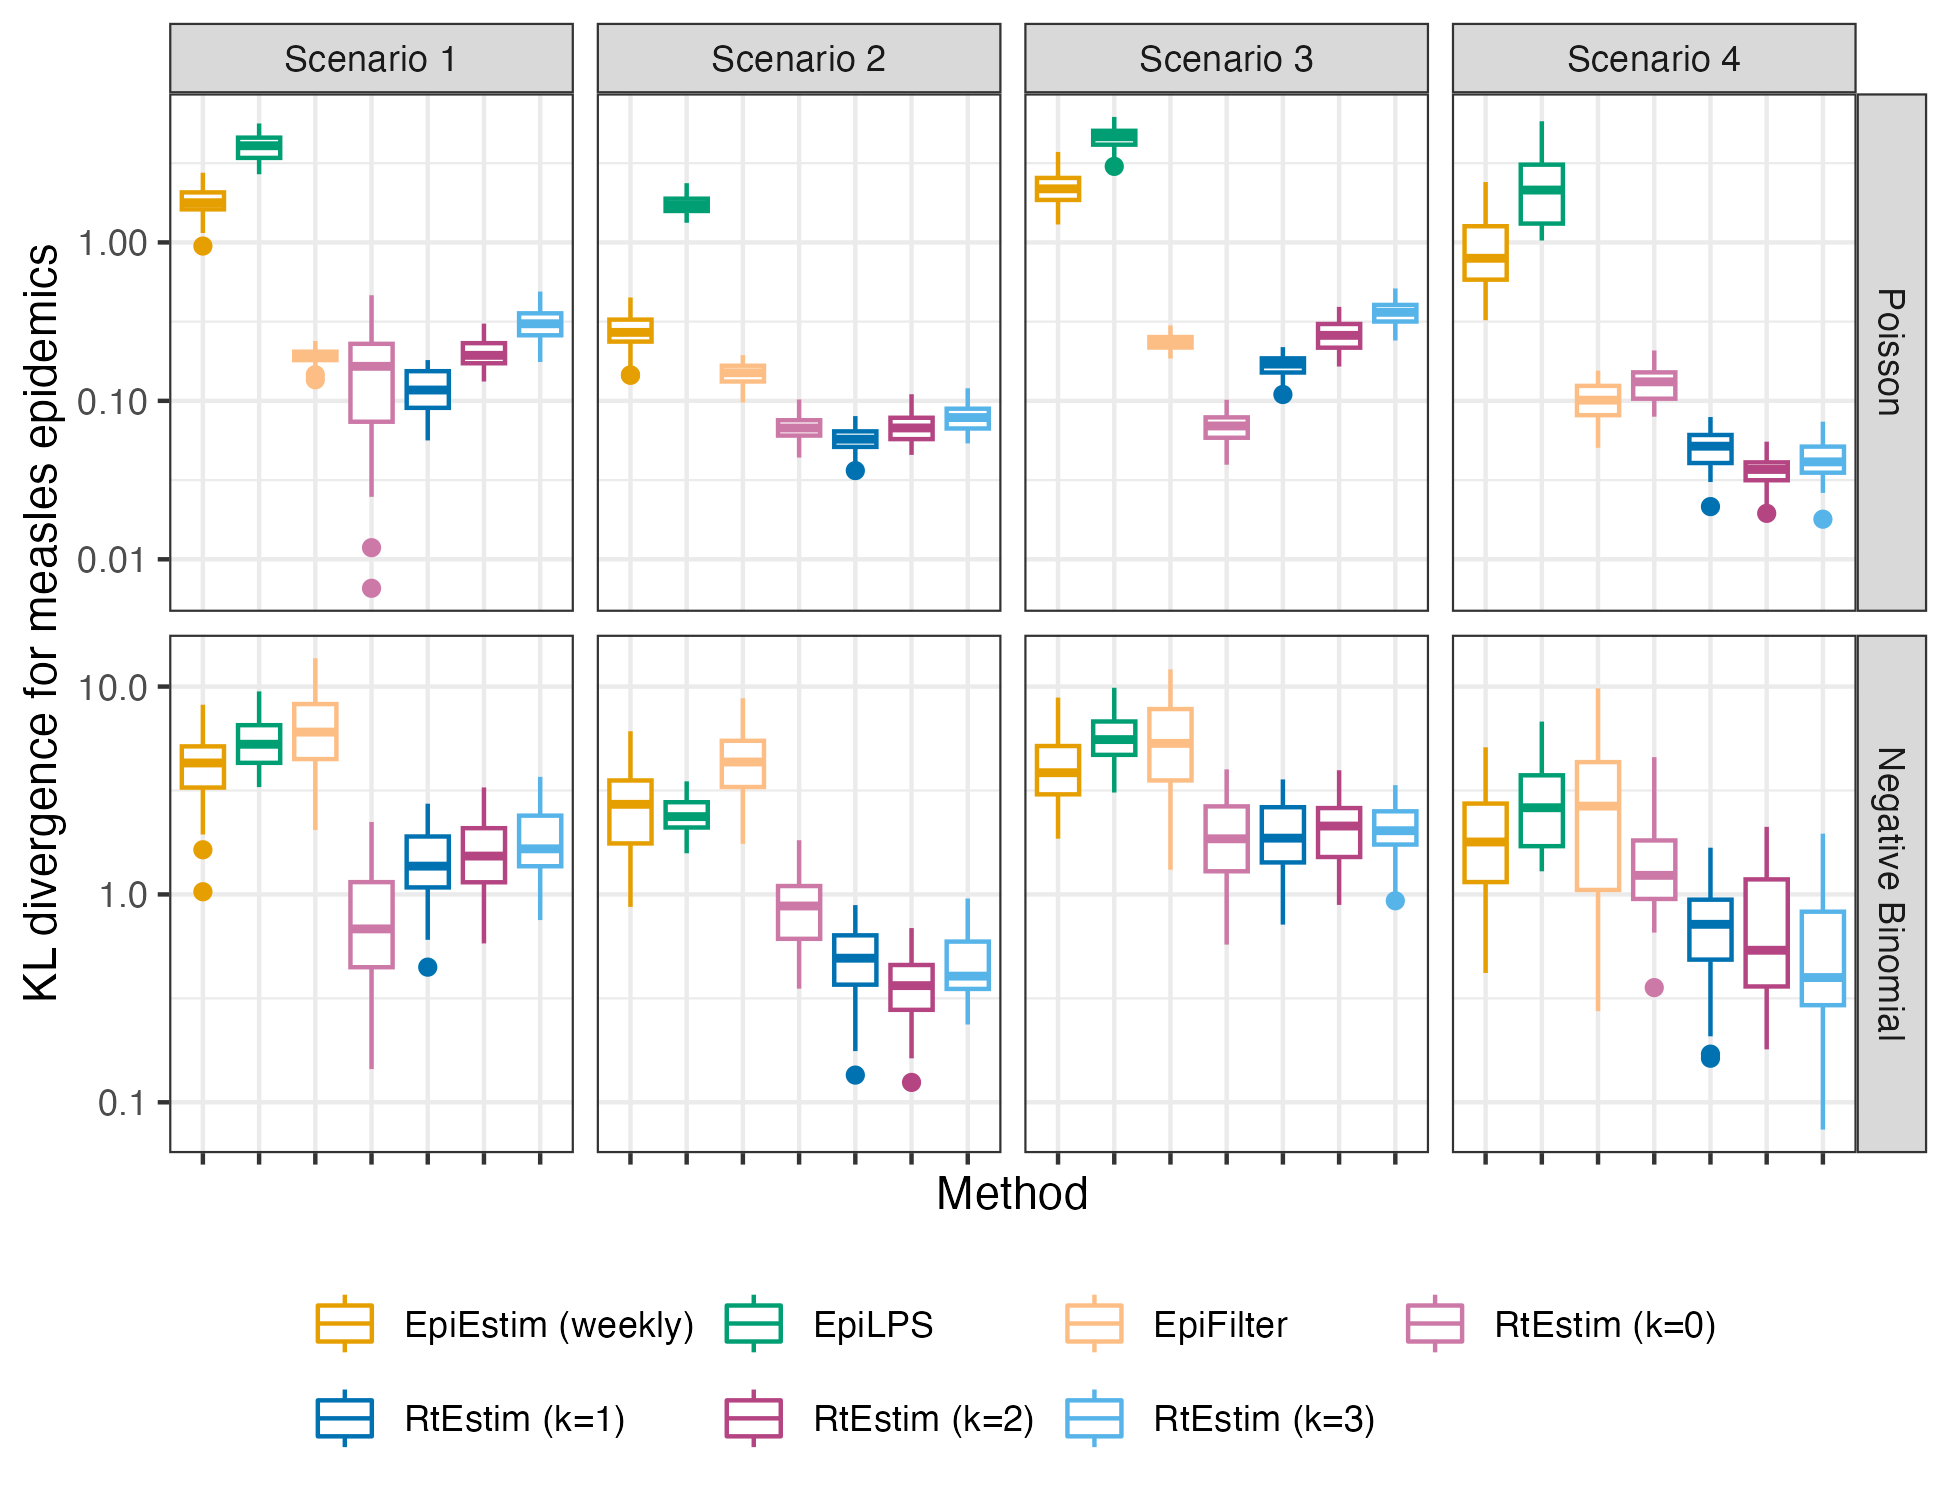
\includegraphics[width=.99\textwidth]{fig/fig_kl_week_measles.png}
  \caption{Boxplot of mean KL divergence between the estimated 
  $\hat{\calR}_t$ and the true $\calR_t$ across 50 synthetic \textbf{measles} epidemics for 
  each approach given Poisson incidence \textit{(in top panels)} and negative 
  binomial incidence \textit{(in bottom panels)} respectively. 
  The mean KL divergence ignores the first weeks in all experiments, since EpiEstim 
  with the weekly sliding window does not provide estimates for the first week.
  Outliers beyond $1.5*$IQR of each box are excluded, and full illustration in 
  provided in the Figure A.3.1 in the supplementary document.} 
  \label{fig:kl-res-measles}
\end{figure}

\begin{figure}[!ht]
  \centering
  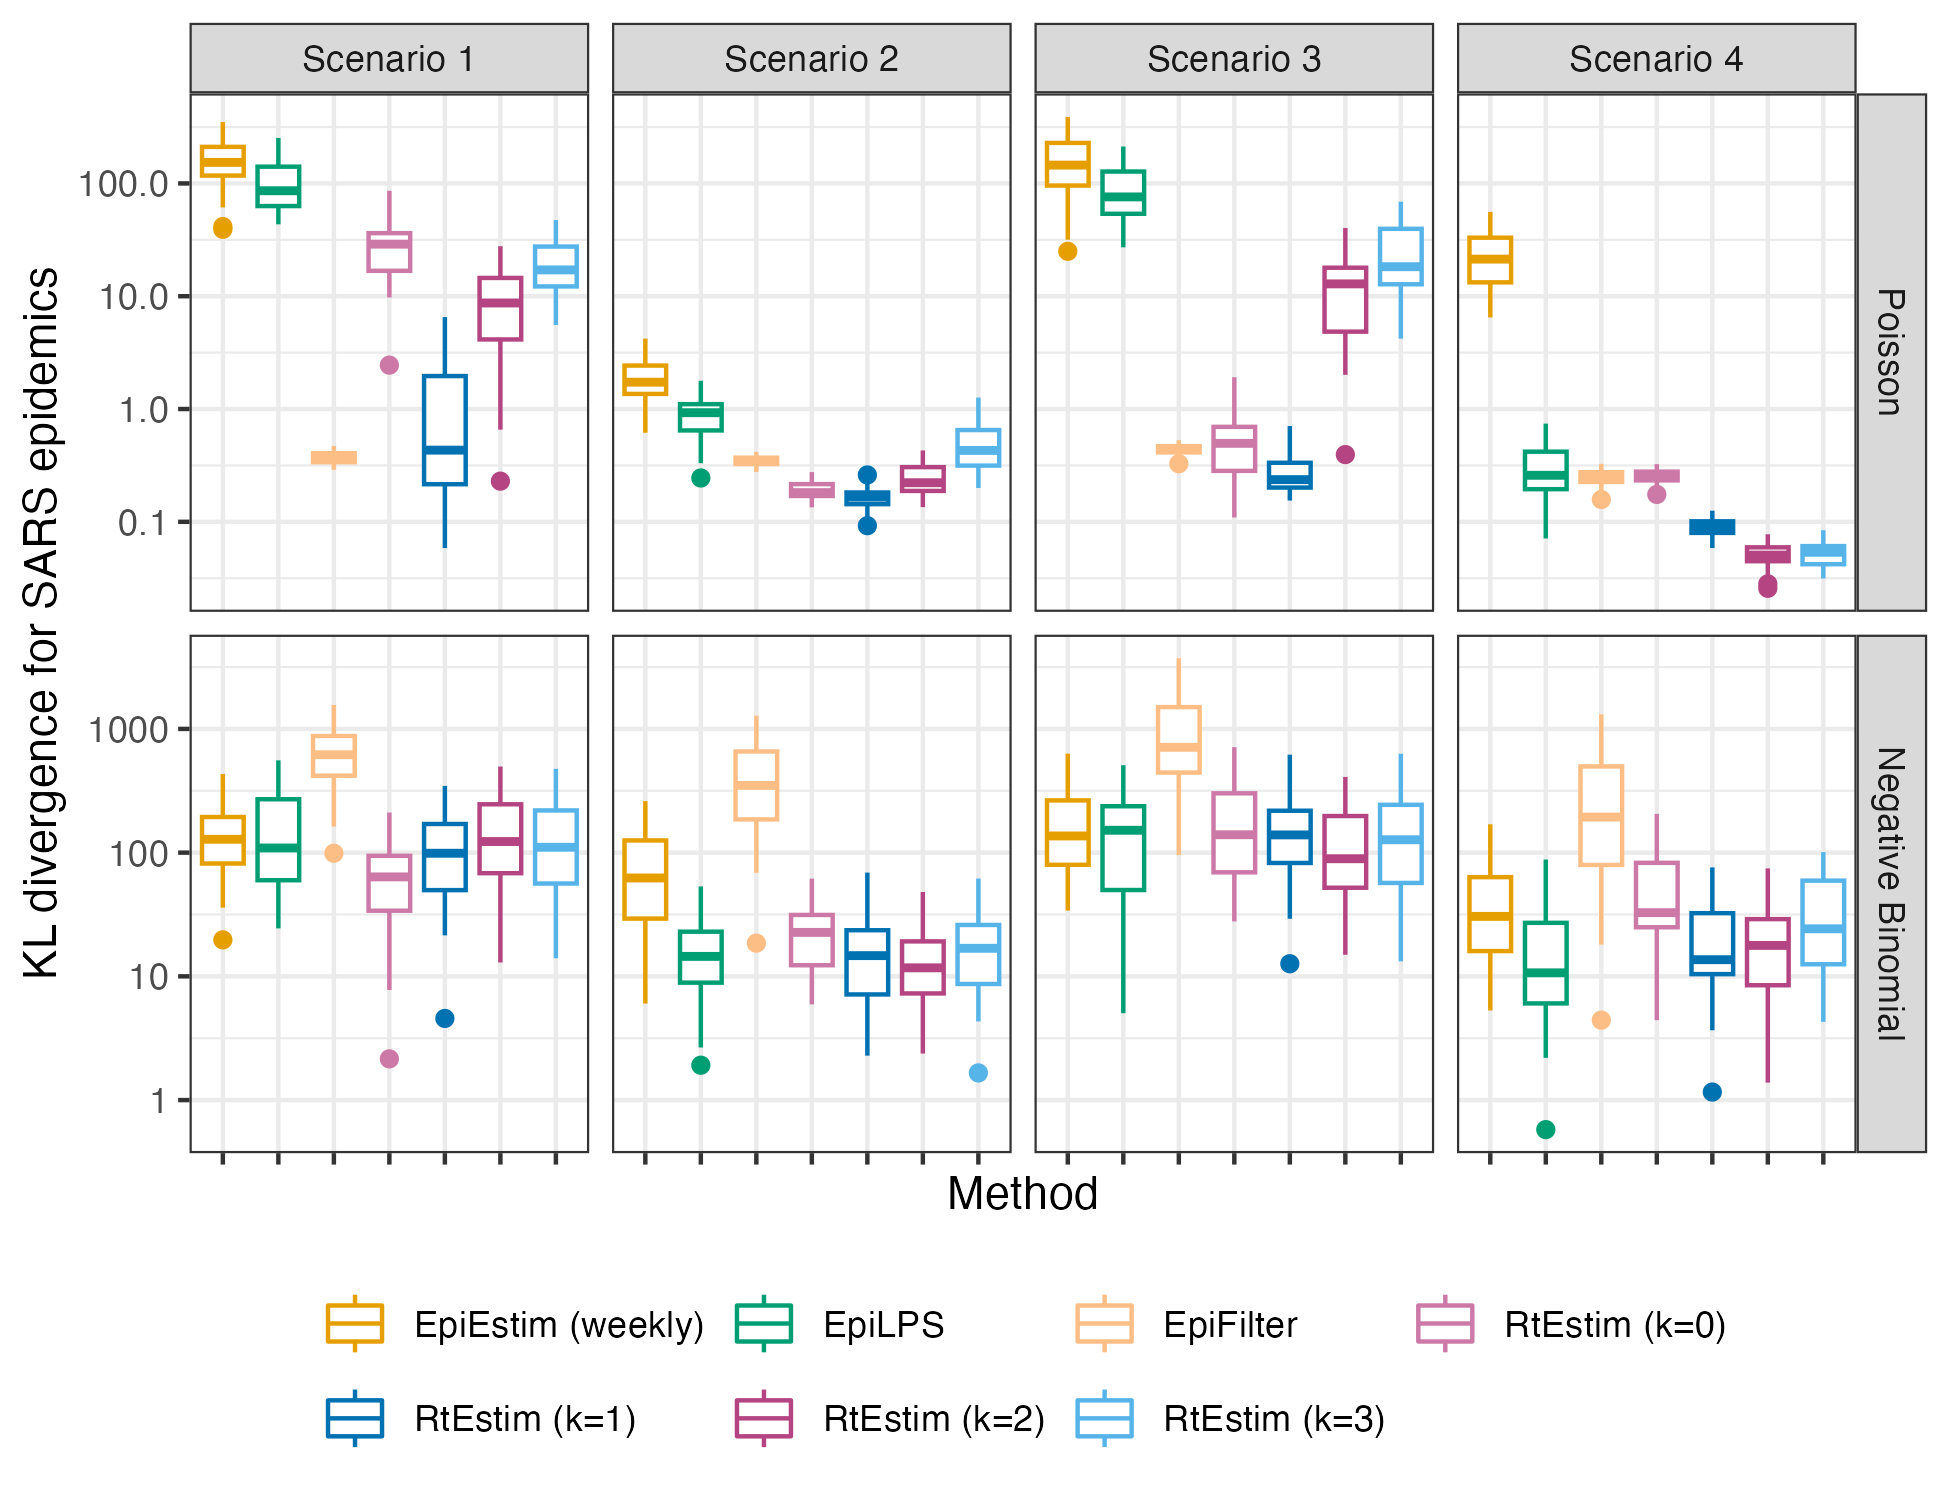
\includegraphics[width=.99\textwidth]{fig/fig_kl_week_sars.png}
  \caption{Boxplot of mean KL divergence between the estimated 
  $\hat{\calR}_t$ and the true $\calR_t$ across 50 synthetic \textbf{SARS} epidemics for 
  each approach given Poisson incidence \textit{(in top panels)} and negative 
  binomial incidence \textit{(in bottom panels)} respectively. 
  The mean KL divergence ignores the first weeks in all experiments, 
  since EpiEstim with the weekly sliding window does not provide estimates 
  for the first week. Outliers beyond $1.5*$IQR of each box are excluded, 
  and full illustration in provided in the Figure A.3.1 in the supplementary document.} 
  \label{fig:kl-res-sars}
\end{figure}

\autoref{fig:pois-est-measles} shows one realization for the estimated effective 
reproduction number under the Poisson generative model in measles synthetic 
epidemics for all four scenarios. An expanded visualization with each estimated 
$\calR_t$ curve displayed in a separate panel is provided in Figure A.6.1 in the supplementary document. 
Ignoring the start of the epidemics, all methods look accurate and recover the 
underlying curves quite well, except \EpiEstim\ with monthly sliding windows, where 
the trajectories are shifted to the right. 
Compared to \EpiEstim\ and \EpiLPS, which have rather severe difficulties at the beginning
of the time series with extremely large estimates at the beginning and decreases rapidly, 
\RtEstim\ and \EpiFilter\ estimates are more accurate without suffering from the 
initialization problem. 
The edge problem in \EpiEstim\ and \EpiLPS\ might be due to the parameters
used in their priors, say the prior mean of $\calR_t$ is initialized to be large, and the incidence
data could not correct it during the beginning of the epidemic.
\RtEstim\ can also have edge problem though, it is less severe in lower orders.
Besides the edge problem, \EpiEstim\ (especially, with the 
monthly sliding window) and \EpiLPS\ produce ``smooth'' estimated curves that are 
continuous at the changepoints in Scenarios 1-3, which results in large mistakes in these neighbourhoods. 
Since the piecewise constant \RtEstim\ estimator does not force any smoothness 
in $\calR_t$, it easily captures the sharp change and nearly overlaps with the 
true values in Scenario 1, and \RtEstim\ with other degrees also well capture 
the correct changepoints. Similar as other methods, \RtEstim\ also suffers from the difficulty to estimate 
the first few timepoints, especially in the periodic scenario, 
where all methods miss to capture the first peak with an accurate value. 
\EpiFilter\ recover the $\calR_t$ curves well in general, but are more wiggly 
than other methods. 


\begin{figure}[!ht]
  \centering
  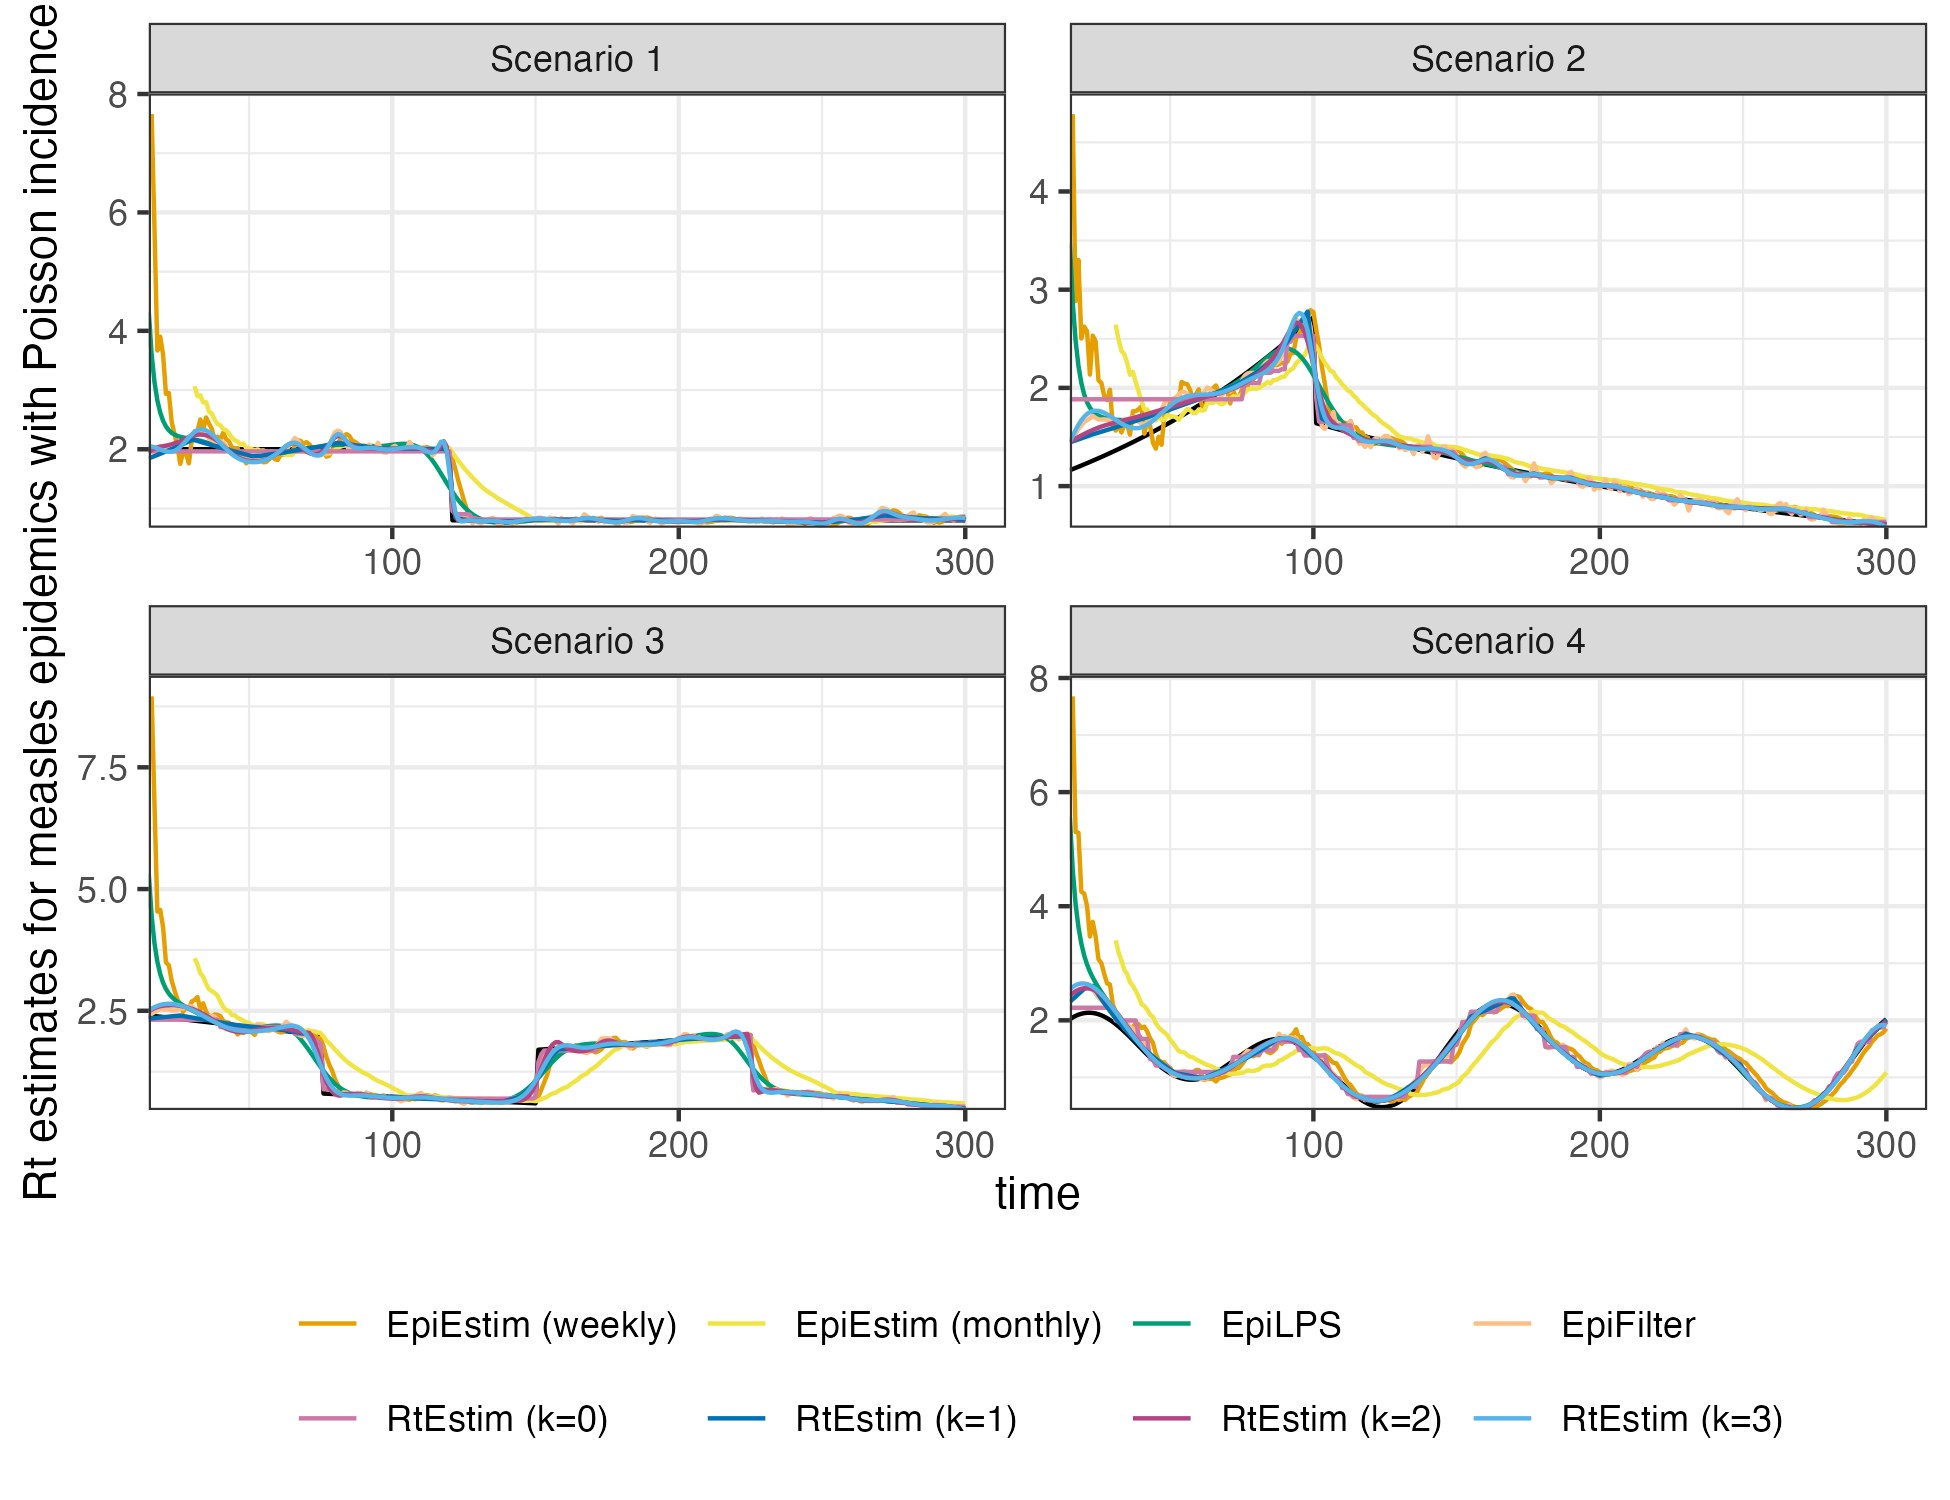
\includegraphics[width=.99\textwidth]{fig/fig_res_pois_measles.png}
  \caption{Example of effective reproduction number estimation for \textbf{measles} 
    epidemics with \textbf{Poisson} observations. An expanded visualization with each estimated 
    $\calR_t$ curve displayed in a separate panel is provided in Figure A.6.1 
    in the supplementary document.}
  \label{fig:pois-est-measles}
\end{figure}

\autoref{fig:nb-est-measles} shows a realization of the estimated $\calR_t$ given
negative binomial incidence in SARS epidemics for each setting. An expanded 
visualization with each estimated $\calR_t$ curve displayed in a separate panel is 
provided in Figure A.6.4 in the supplementary document. Compared to the measles epidemics 
with Poisson data, all methods perform worse overall for SARS epidemics with negative 
binomial incidence due to two possible reasons, larger incidence and overdispersed data. 
The challenges to recover the start of epidemics are even harder in this setting for 
all methods. \EpiFilter\ has much more wiggly estimates in this setting than the estimates of other 
methods compared to the setting in \autoref{fig:pois-est-measles}. Our \RtEstim\ 
estimates are close to the best performance in the first three $\calR_t$ scenarios, 
while face the challenge to recover the curve in the periodic scenario. 

%To investigate the performance when the Poisson assumption (imposed by both
%\RtEstim\ and \EpiEstim) is violated, we also examine estimation accuracy with
%negative binomial data. \autoref{fig:nb-est-measles} displays a realization, analogous
%to the previous case, for all methods and scenarios. \RtEstim\ has more
%difficulty relative to the Poisson setting, especially at the beginning of the
%outbreak. This is most pronounced in Scenario 4, where \RtEstim\ is overly
%smooth, except in the last wave. In Scenario 2, \RtEstim\ successfully captures
%the changepoint, but suffers from the same discontinuity problem as in the
%Poisson setting. In Scenario 3, the piecewise linear version of \RtEstim\
%recovers the curvature of $\calR_t$ well, but is less accurate than in the
%Poisson case. 

\begin{figure}[!ht]
  \centering
  \includegraphics*[width=.99\textwidth]{fig/fig_res_NB_sars.png}
  \caption{Example of effective reproduction number estimation for \textbf{SARS} 
  epidemics with \textbf{negative binomial} observations. An expanded visualization 
  with each estimated $\calR_t$ curve displayed in a separate panel is provided 
  in Figure A.6.4 in the supplementary document.}
  \label{fig:nb-est-measles}
\end{figure}

Finally, it is important to provide a brief comparison of the running times of
all three models across the $8$ experimental settings. We find that almost all
models across all experiments complete within $10$ seconds. \RtEstim\ generally
takes the longest, due to a relatively large number of estimates---$50$ values
of $\lambda$ and $10$ folds of cross validation require $550$ estimates---while
other models run only a single time for a fixed setting of hyperparameters per
experiment. Additional results on timing comparisons are deferred to the
supplementary document. 


\subsection{Real-data results: Covid-19 incident cases in Canada}

We implement \RtEstim\ on Covid-19 confirmed incident cases in Canada (visualized in 
\autoref{fig:intro-fig}). 
We use the weighted probabilities of serial interval distributions of four dominant
variants used in \autoref{fig:intro-fig} as the serial interval distribution here for the
comparison with other methods, which cannot incorporate time-varying serial interval distributions. 
We compute their percentages of days that they dominated throughout the pandemic as the weights in computation, 
specifically Ancestral lineage ($32.6\%$), Alpha ($8.5\%$), Delta ($16.0\%$), and Omicron($42.9\%$) with sum 1. 
The estimates of our method is displayed in \autoref{fig:covid-rt}, and the estimates of 
all competitors are deferred to Figures A.8.1 and A.8.2 in the supplementary document. 

Considering the first, second, and third polynomial degrees, $\widehat{\calR}_t$
for Covid-19 in Canada is
always less than $2$ except at the very early stage, which means that one
distinct infected individual on average infects less than two other
individuals in the population. Examining three different settings for $k$, the
temporal evolution of $\widehat{\calR}$ (across all regularization levels
$\lambda$) are similar near the highest peak around the end of 2021 before
dropping shortly thereafter. Throughout the estimated curves, the peaks and
troughs of the effective reproduction numbers precede the growth and decay cycles of
confirmed cases, as expected. We also visualize 95\% confidence bands for the
point estimates with $\lambda$ chosen by minimizing cross-validated KL
divergence in \autoref{fig:covid-rt}.     

\begin{figure}[!ht]
  \centering
  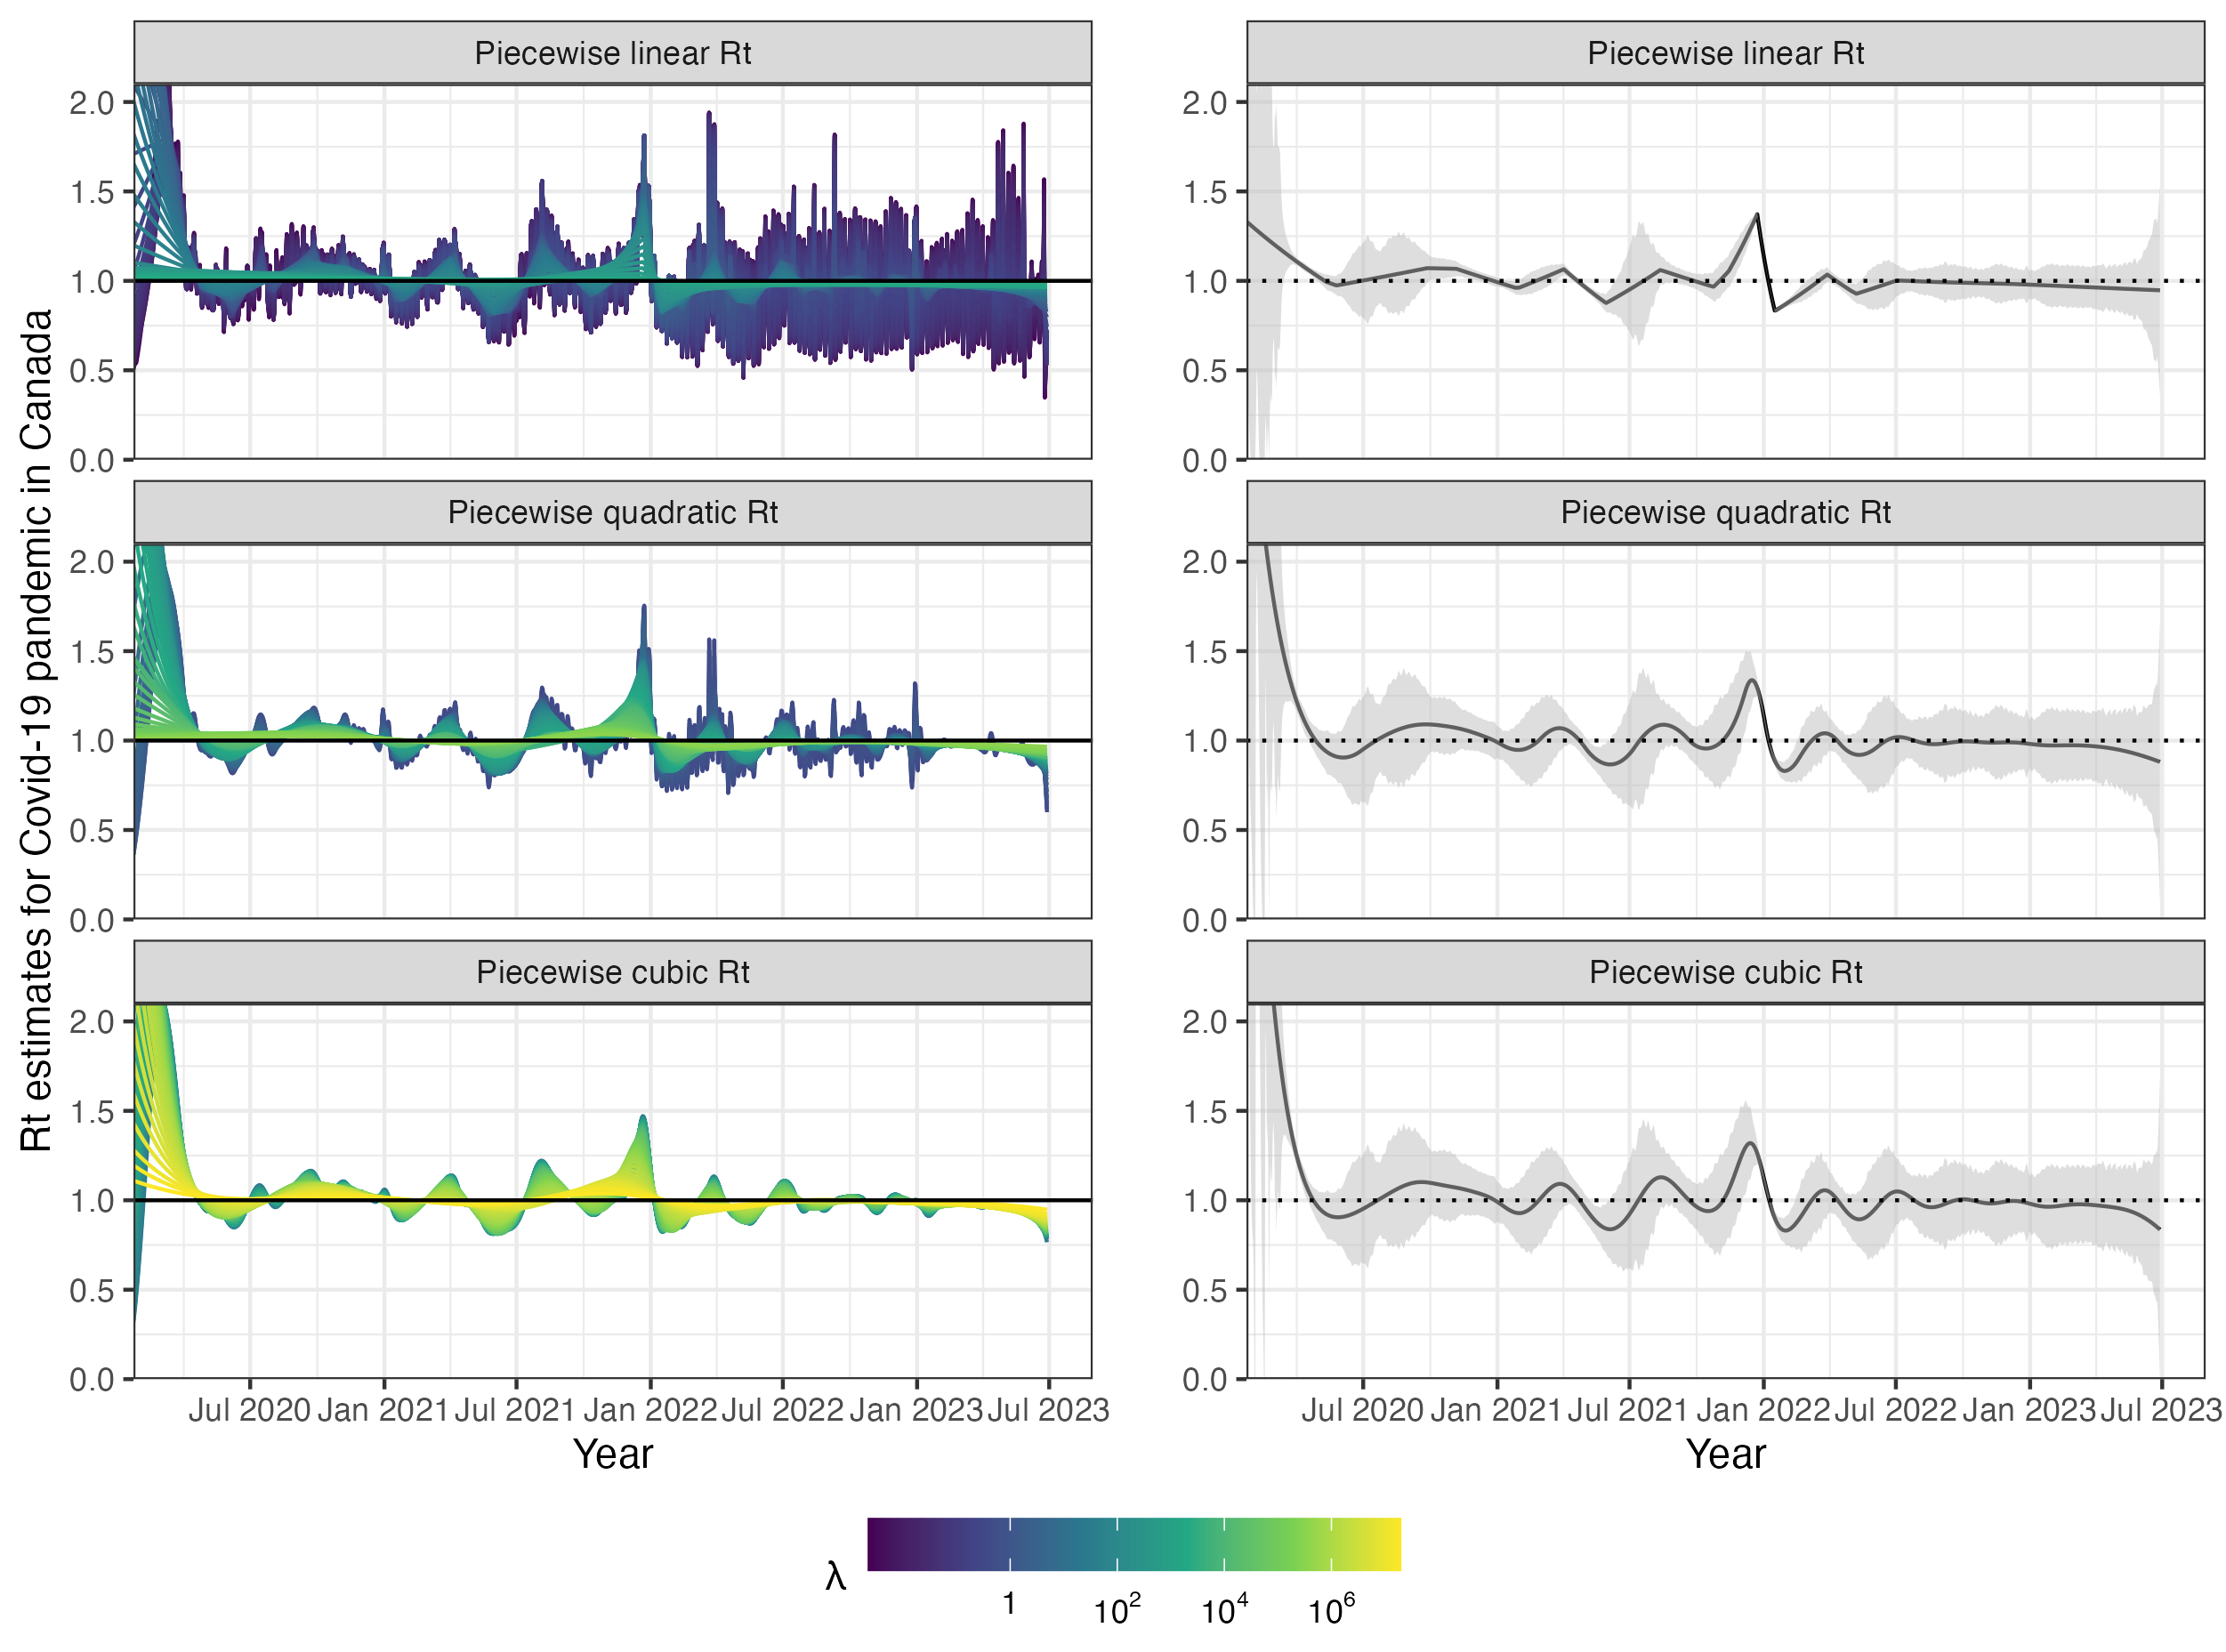
\includegraphics[width=0.99\linewidth]{fig/covid_full_res.png}
  \caption{Estimated effective reproduction number based on Covid-19 daily
  confirmed incident cases between January 23rd, 2020 and June 28th, 2023 in
  Canada. The left panels show estimates corresponding to 50
  tuning parameters. The right panels show the CV-tuned estimate along with
  approximate 95\% confidence bands. The top, middle and bottom panels show the
  estimated $\calR_t$ using the Poisson trend filtering in \eqref{eq:rt-ptf}
  with degrees $k=1,2,3$ respectively. All estimates are fitted using a constant
  serial interval distribution, which is the weighted sum of probabilities of 
  the 4 dominant variants per timepoint used in \autoref{fig:intro-fig}. 
  All panels are truncated in y-axes for better illustration. The CV-tuned 
  $\calR_t$ estimates rapidly decrease at the early stage from $3.37,5.16$ 
  in $\calR_t$ curves with $k=2,3$ respectively.} 
  \label{fig:covid-rt}
\end{figure} 

The estimated effective reproduction numbers are relatively unstable before April,
2022. The highest peak coincides with the emergence and global spread of the
Omicron variant. The estimated effective reproduction numbers fall below 1 during 
a few time periods, where the most obvious troughs are roughly from April 2021 to July 2021 and from January,
2022 to April 2022. The first trough coincides with the introduction of
Covid-19 vaccines in Canada. The second trough, shortly after the
largest peak may be due to variety of factors resulting in the depletion of the
susceptible population such as increased self-isolation in response to media
coverage of the peak or immunity incurred via recent infection. Since April
2022, the estimated effective reproduction number has remained relatively stable
(fluctuating around one) corresponding to low reported cases, though reporting
behaviours also changed significantly since the Omicron wave. 


\subsection{Real-data results: influenza in Baltimore, Maryland, 1918}

We also apply \RtEstim\ to daily reported influenza cases in Baltimore, Maryland
occurring during the world-wide pandemic of 1918 from September to November 
\citep{frost1919influenza}. The
data, shown in \autoref{fig:flu-dat}, is included in the \EpiEstim\ \R\ package.
We use the serial interval distribution provided by the \EpiEstim\ \R\ package for
this pandemic in modelling. 
The 1918 influenza outbreak, caused by the H1N1 influenza A virus, was
unprecedentedly deadly with case fatality rate over 2.5\%, infecting almost
one-third of the population across the world \citep{taubenberger20061918}. The
CV-tuned piecewise cubic estimates in \autoref{fig:flu-res} better capture the
growth at the beginning of the pandemic in \autoref{fig:flu-dat}. The estimated
$\calR_t$ curve suggests that the transmissibility of the pandemic grew rapidly
over the first 30 days before declining below one after 50 days. However, it
also suggests an increase in infectiousness toward the end of the period. With
this data, it is difficult to determine if there is a second wave or a steady
decline ahead. The CV-tuned piecewise constant and linear estimates in
\autoref{fig:flu-res} both suggest a steady decline. This conclusion is
supported by the fact that incident cases decline to zero at the end of the
period and matches $\calR$ estimates in \cite{cori2013new}, which are all lower
than one.
The estimation using alternatives is deferred to Figures A.8.3 and A.8.4 
in the supplementary document.

\begin{figure}[!ht]
  \centering
  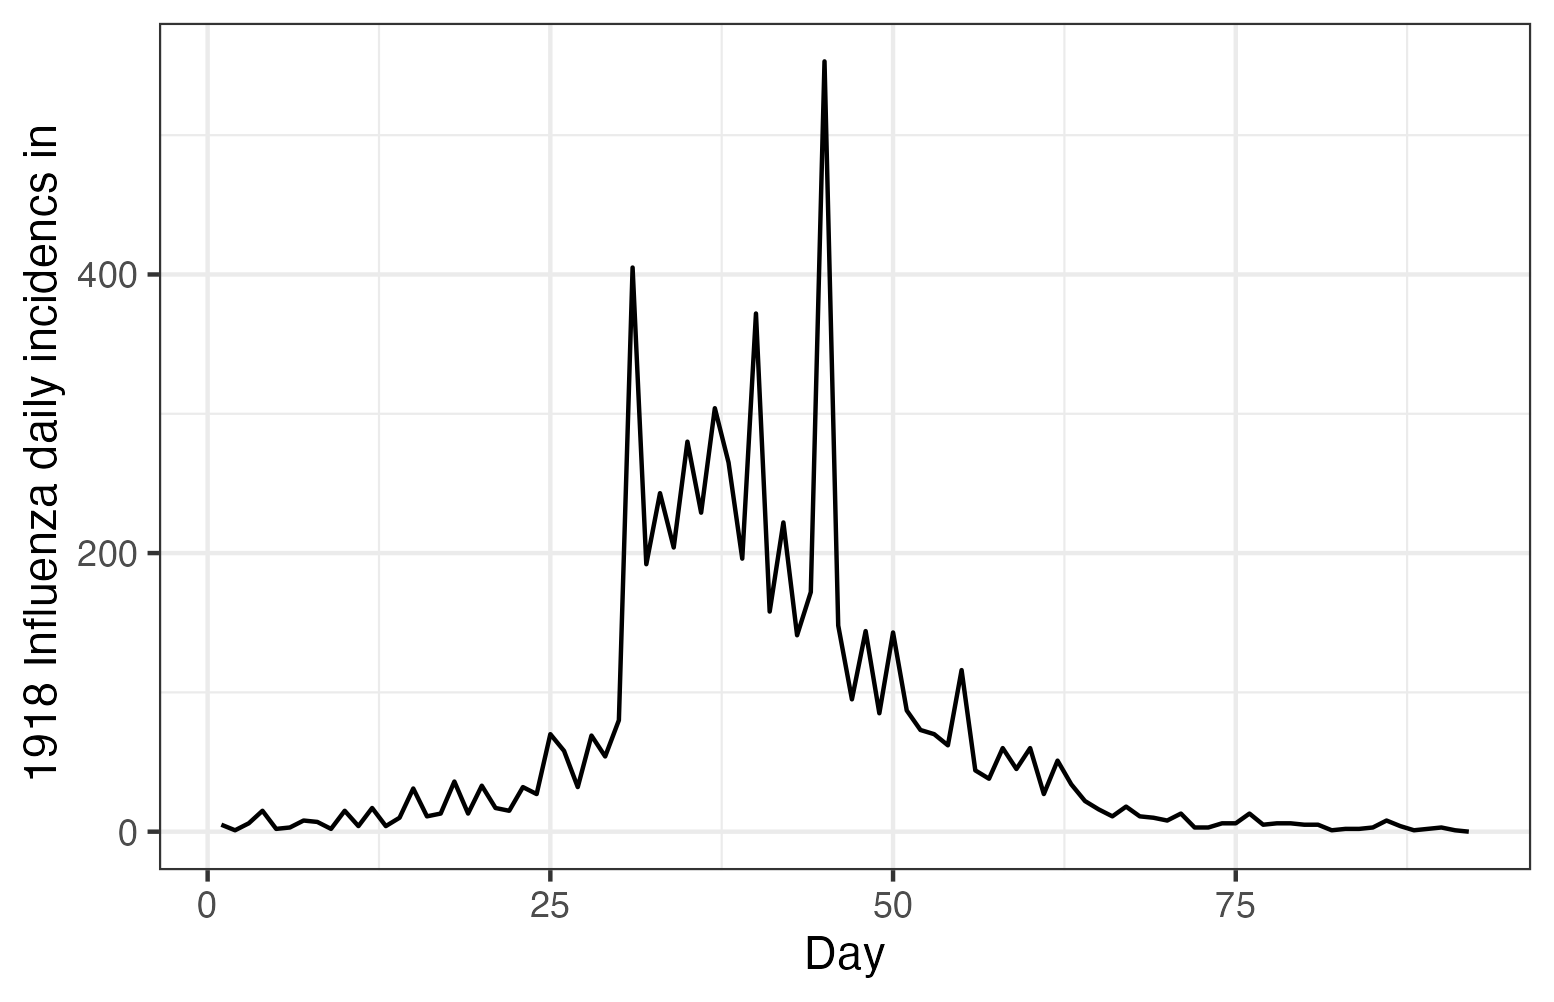
\includegraphics[width=0.8\linewidth]{fig/flu_dat.png}
  \caption{Daily incident influenza cases in Baltimore, Maryland between September 
  and November in 1918.} 
  \label{fig:flu-dat}
\end{figure} 

\begin{figure}[!ht]
  \centering
  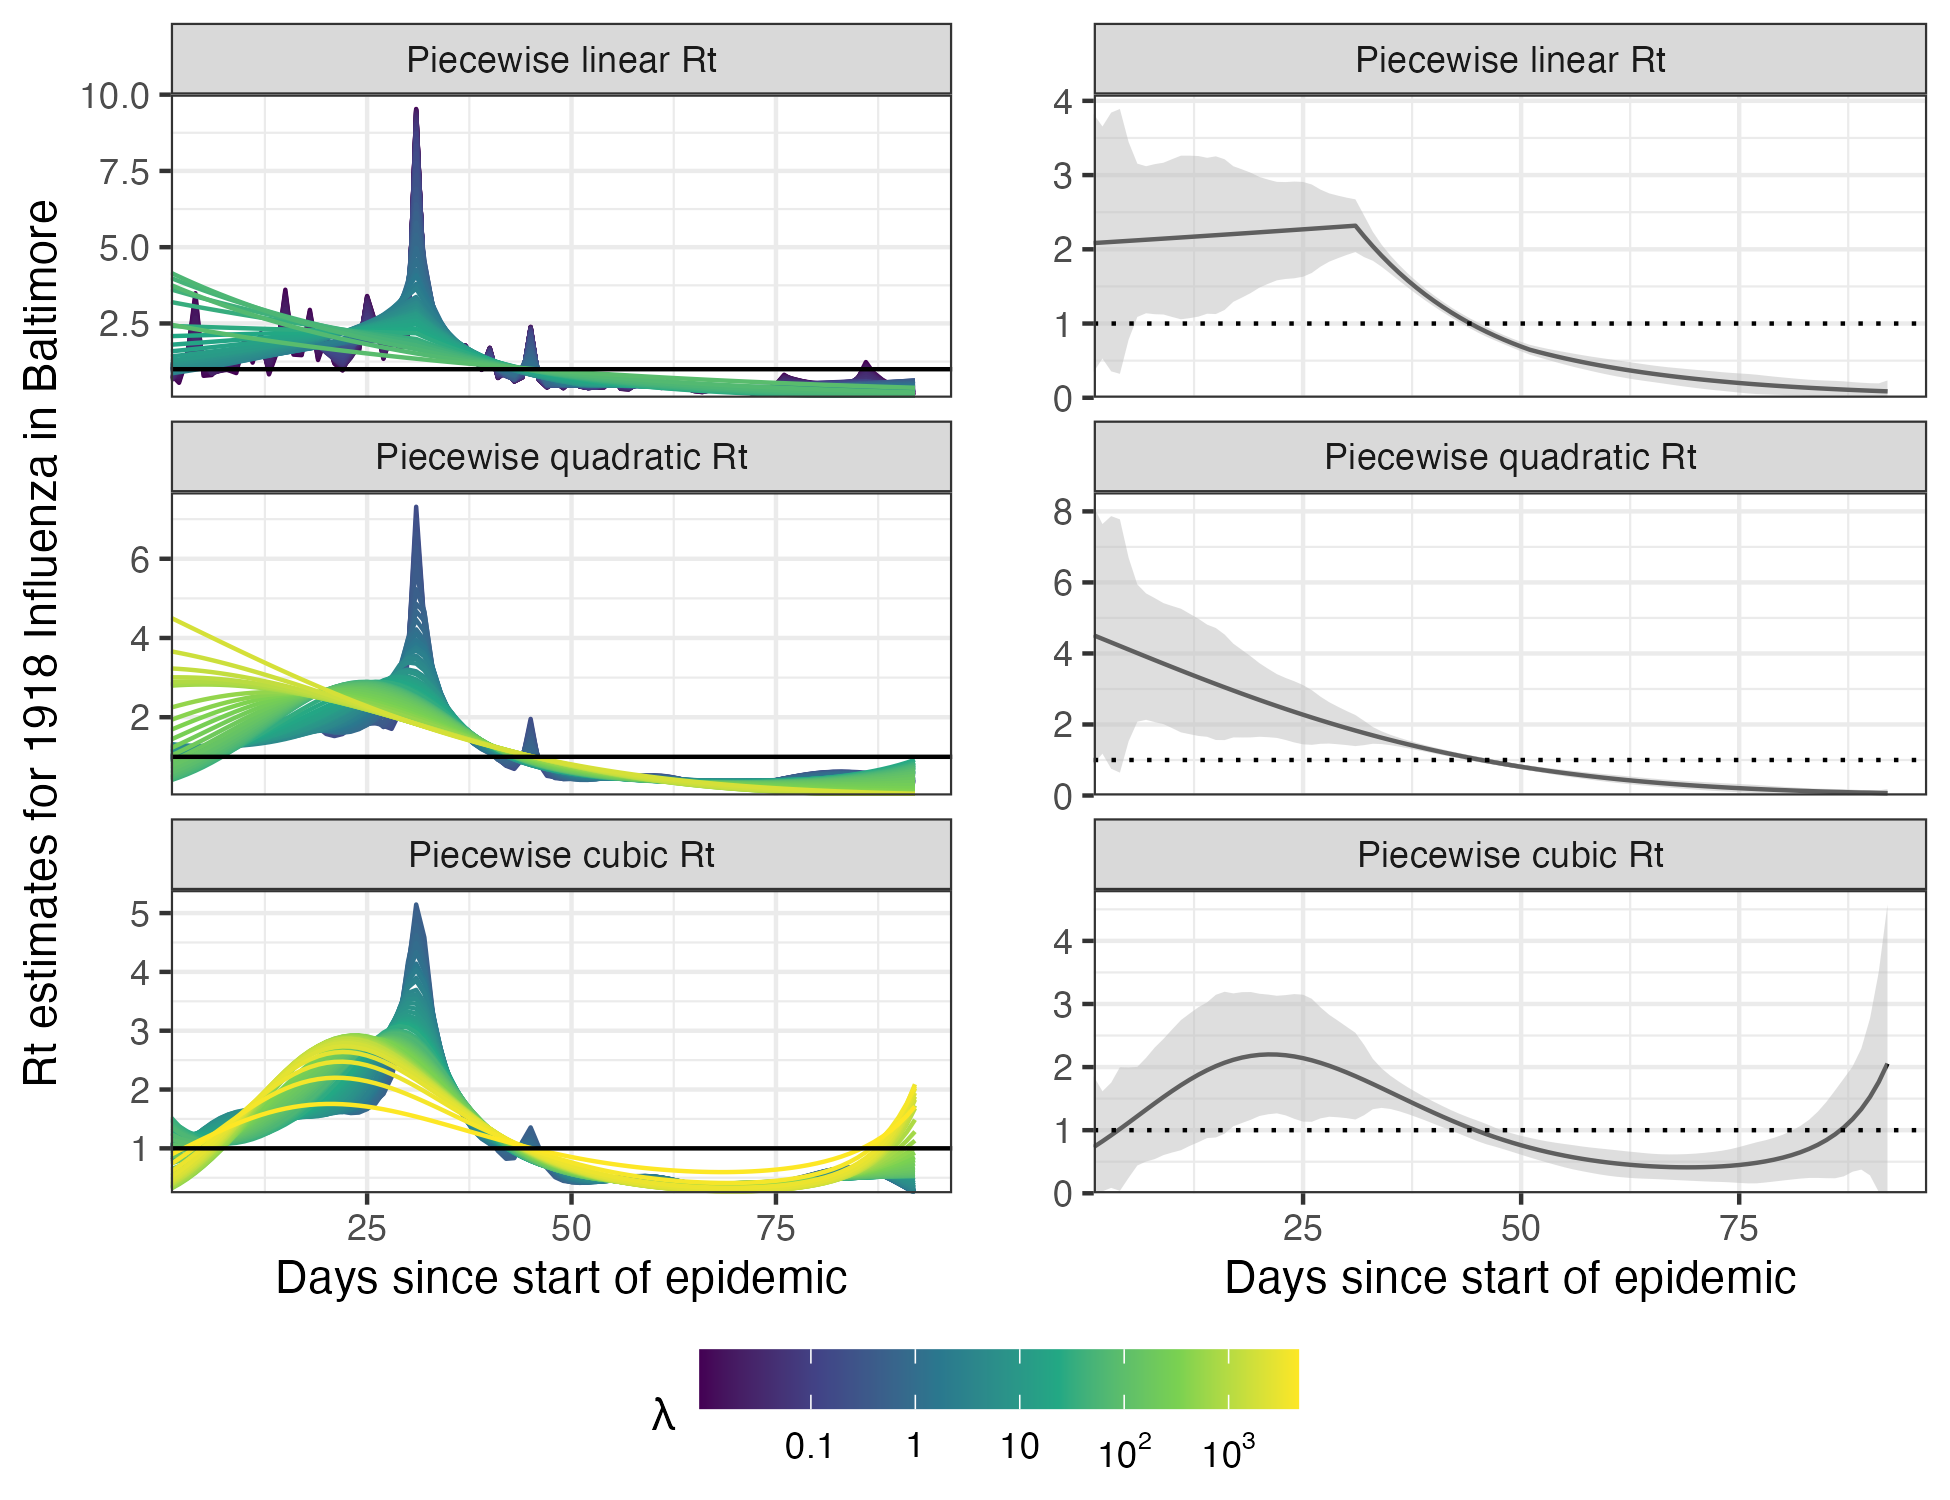
\includegraphics[width=0.99\linewidth]{fig/flu_full_res.png}
  \caption{Estimated effective reproduction numbers for influenza in Baltimore,
  Maryland in 1918. The left panels show estimates for a set of 50 tuning
  parameters. The right column displays the CV-tuned estimates with approximate
  95\% confidence bands. The rows (top to bottom) show estimated effective reproduction
  numbers ($\calR_t$) using the Poisson trend filtering in \eqref{eq:rt-ptf}
  with $k=1,2,3$ respectively.} 
  \label{fig:flu-res}
\end{figure} 


\section{Discussion}
\label{sec:disc}

The \RtEstim\ methodology provides a locally adaptive estimator using Poisson
trend filtering on univariate data. It captures the heterogeneous smoothness of
effective reproduction numbers given observed incidence data rather than
resulting in global smoothness. This is a nonparametric regression model which
can be written as a convex optimization (minimization) problem. Minimizing the
distance (KL divergence across all coordinates) between the estimators and
(functions of) observations guarantees data fidelity while the penalty on divided
differences between pairs of neighbouring parameters imposes smoothness. The
$\ell_1$-regularization results in sparsity of the divided differences, which
leads to heterogeneous smoothness across time. 


The property of local adaptivity (heterogenous smoothness) is useful to
automatically distinguish, for example, seasonal outbreaks from outbreaks driven
by other factors (behavioural changes, foreign introduction, etc.). Given a
well-chosen polynomial degree, the growth rates can be quickly detected, 
potentially advising public health authorities to implement policy changes. The effective
reproduction numbers can be estimated retrospectively to examine the efficacy of
such policies, whether they result in $\calR_t$ falling below 1 or the speed of
their effects. The smoothness of $\calR_t$ curves (including the polynomial 
degrees and tuning parameters) should be chosen based on the purpose of the 
study in practice. 


Our method \RtEstim\ provides a natural way to deal with missing data, for
example, on weekends and holidays or due to changes in reporting frequency.
While solving the convex optimization problem, our method can easily 
handle uneven spacing or irregular reporting. Computing the total
primary infectiousness is also easily generalized to irregular reporting by
modifying the discretization of the serial interval distribution. There are many
other aspects to be considered in choosing the delay distribution to make a more accurate
estimation \citep{park2024estimating}. 
Imported cases can be distinguished from the local cases to avoid the biasness 
in effective reproduction number estimation, for example, \cite{thompson2019improved} 
assumed the total past infectiousness of combined previous cases scaled by effective 
reproduction number to be the mean of the local incidence and illustrated that 
failure of distinguishing the local cases from the imported cases may cause the overestimation 
of $\calR$ using the MERS data in Saudi Arabia from August 2014 to December 2015. 
Additionally, because the $\ell_1$ penalty introduces sparsity (operating like a median
rather than a mean), this procedure is relatively insensitive to outliers
compared to $\ell_2$ regularization.


There are a number of limitations that may influence the quality of
$\calR_t$ estimation. While our model is generic for incidence data 
rather than tailored to any specific disease, it does assume that the 
generation interval is short relative to the period of data collection. 
More specialized methodologies would be required for diseases with long 
incubation periods such as HIV or Hepatitis. 
Our approach, does not explicitly model imported cases, nor distinguish between
subpopulations that may have different mixing behaviour. 
While the Poisson assumption is common, it does not handle overdispersion
(observation variance larger than the mean). The negative binomial distribution
is a good alternative, but more difficult to estimate in this context.
As described in \autoref{sec:intro}, the expression for $\calR$ 
assumes that a relatively constant proportion of true infections is reported. 
However, if this proportion varies with time (say, due to changes in surveillance
practices or testing recommendations), the estimates may be biased over this
window. A good example is in early January 2022, during the height of the
Omicron wave, Canada moved from testing all symptomatic individuals to
testing only those in at-risk groups. The result was a sudden change that would
render $\calR_t$ estimates on either side of this timepoint incommensurable.


Our \RtEstim\ implementation can take a fixed serial interval throughout the
period of study (as implemented in simulation and in the real epidemics) or 
varying serial interval distributions at different timepoints (as implemented 
in \autoref{fig:intro-fig} for Covid-19 data in Canada). In reality, the serial
interval may vary due to changes in the factors such as population immunity 
\citep{nash2023estimating}. An issue regarding the serial interval distribution 
relates to equating serial and generation intervals (also mentioned above). 
The serial interval distribution is generally wider than that 
of the generation interval, because the serial interval involves the convolution
of two distributions, and is unlikely to actually follow a named distribution
like Gamma, though it may be reasonably well approximated by one. Our
implementation allows for an arbitrary distribution to be used, but requires the
user to specify the discretization explicitly, requiring more nuanced knowledge
than is typically available. Pushing this analysis further, to accommodate other
types of incidence data (hospitalizations or deaths), a modified generation
interval distribution would be necessary, and further assumptions would be
required as well. Or else, one would first need to deconvolve deaths to
infection onset before using our software.


Accurate statistical coverage of a function is a difficult problem, and the
types of (frequentist) guarantees that can be made are not always what one
would want \citep{genovese2008adaptive}. We examine the coverage of our 
approximate confidence interval in simulation. (Details are deferred to Section A.6 
in the supplementary document). Empirically, our observations for our method, as well 
as all others we have seen, follow a similar (undesirable) pattern: when 
$\mathcal{R}_t$ is stable, they \emph{over cover} dramatically (even implausibly 
narrow intervals have 100\% coverage); but when $\mathcal{R}_t$ changes abruptly, 
they \emph{under cover} (coverage drops to nearly 0\%). 
Theoretically, whether these intervals should be expected to provide $(1-\alpha)\%$ 
coverage simultaneously over all time while being narrow enough to provide useful
uncertainty quantification is neither easy nor settled. 


Nonetheless, our methodology is implemented in a lightweight \R\ package 
\texttt{rtestim} and computed efficiently, especially for large-scale data, 
with a proximal Newton solver coded in \cpp. 
Given available incident case data, prespecified serial interval
distribution, and a choice of degree $k$, \RtEstim\ is able to produce
accurate estimates of effective reproduction number and provide efficient
tuning parameter selection via cross validation. 


%\section*{Supporting information}
%
%% Include only the SI item label in the paragraph heading. Use the \nameref{label} command to cite SI items in the text.
%\paragraph*{Fig 1.}
%\label{fig:intro-fig}
%{\bf A demonstration of effective reproduction number estimation 
%by \RtEstim\ and the corresponding fitted incident cases for the Covid-19 epidemic 
%in Canada during a period from March 28, 2020 to June 28, 2023.}
%The blue curve in the top panel is the estimated piecewise
%quadratic $\calR_t$ and the gray ribbon is the corresponding 95\% confidence band. 
%The black curve in the bottom panel is the observed Covid-19 daily confirmed 
%cases, and the orange curve is the fitted incidence 
%corresponding to the estimated $\calR_t$.
%
%\paragraph*{Fig 2.}
%\label{fig:samples}
%{\bf The effective reproduction numbers (left column) and corresponding
%sample incident cases drawn from a Poisson (middle column) or negative
%Binomial (right column) distribution.} The rows correspond to the four
%$\calR_t$ settings.
%
%\paragraph*{Fig 3.}
%\label{fig:kl-res}
%{\bf Boxplot of KL divergence between the estimated 
%$\hat{\calR}_t$ and the true $\calR_t$ across 50 random samples for 
%each approach given Poisson incidence \textit{(in top panels)} and negative 
%Binomial incidence \textit{(in bottom panels)} respectively.}  
%Outliers are excluded. Full visualization is deferred to the \nameref{Appendix}.
%
%\paragraph*{Fig 4.}
%\label{fig:pois-est}
%{\bf Example of effective reproduction number estimation for Poisson incidence.}
%
%\paragraph*{Fig 5.}
%\label{fig:nb-est}
%{\bf Example of effective reproduction number estimation for negative Binomial
%incidence.}
%
%\paragraph*{Fig 6.}
%\label{fig:covid-data}
%{\bf Covid-19 daily confirmed incident cases between March 1st, 
%2020 and April 15th, 2023 in Canada.}
%
%\paragraph*{Fig 7.}
%\label{fig:covid-rt}
%{\bf Estimated effective reproduction numbers for Covid19 daily confirmed 
%counts between March 1st, 2020 and April 15th, 2023 in Canada.} 
%The left panels demonstrate estimates corresponding to 50 tuning parameters. 
%The right panels display the CV-tuned estimates with 95\% confidence intervals. 
%The top, medium and bottom panels illustrate the estimated reproduction numbers 
%($\calR_t$) using the Poisson trend filtering (in \eqref{eq:rt-ptf}) with 
%degrees $k=1,2,3$ respectively.
%
%\paragraph*{Fig 8.}
%\label{fig:flu-dat}
%{\bf Daily influenza incident counts in Baltimore, Maryland between September 
%and November in 1918.}
%
%\paragraph*{Fig 9.}
%\label{fig:flu-res}
%{\bf Estimated effective reproduction numbers for influenza in
%Baltimore, Maryland in 1918.} The left panels show estimates for all
%50 tuning parameters under consideration. The right column displays the 
%CV-tuned estimates with 95\% confidence bands. The rows (top to bottom) show
%estimated reproduction numbers ($\calR_t$) using the Poisson trend filtering
%(in \eqref{eq:rt-ptf}) with degrees $k=1,2,3$ respectively.
%
%\paragraph*{Appendix.}
%\label{Appendix}
%{\bf Supplementary details on methodology and experiments of effective 
%reproduction number estimation with trend filtering.} 


\section*{Acknowledgments}

This research was enabled in part by support provided by 
BC DRI group who manages Cedar cloud (https://docs.alliancecan.ca/wiki/Cedar)
and the Digital Research Alliance of Canada (alliancecan.ca).

\nolinenumbers

% Either type in your references using
% \begin{thebibliography}{}
% \bibitem{}
% Text
% \end{thebibliography}
%
% or
%
% Compile your BiBTeX database using our plos2015.bst
% style file and paste the contents of your .bbl file
% here. See http://journals.plos.org/plosone/s/latex for 
% step-by-step instructions.
% 
\bibliography{doc/ptf}

 

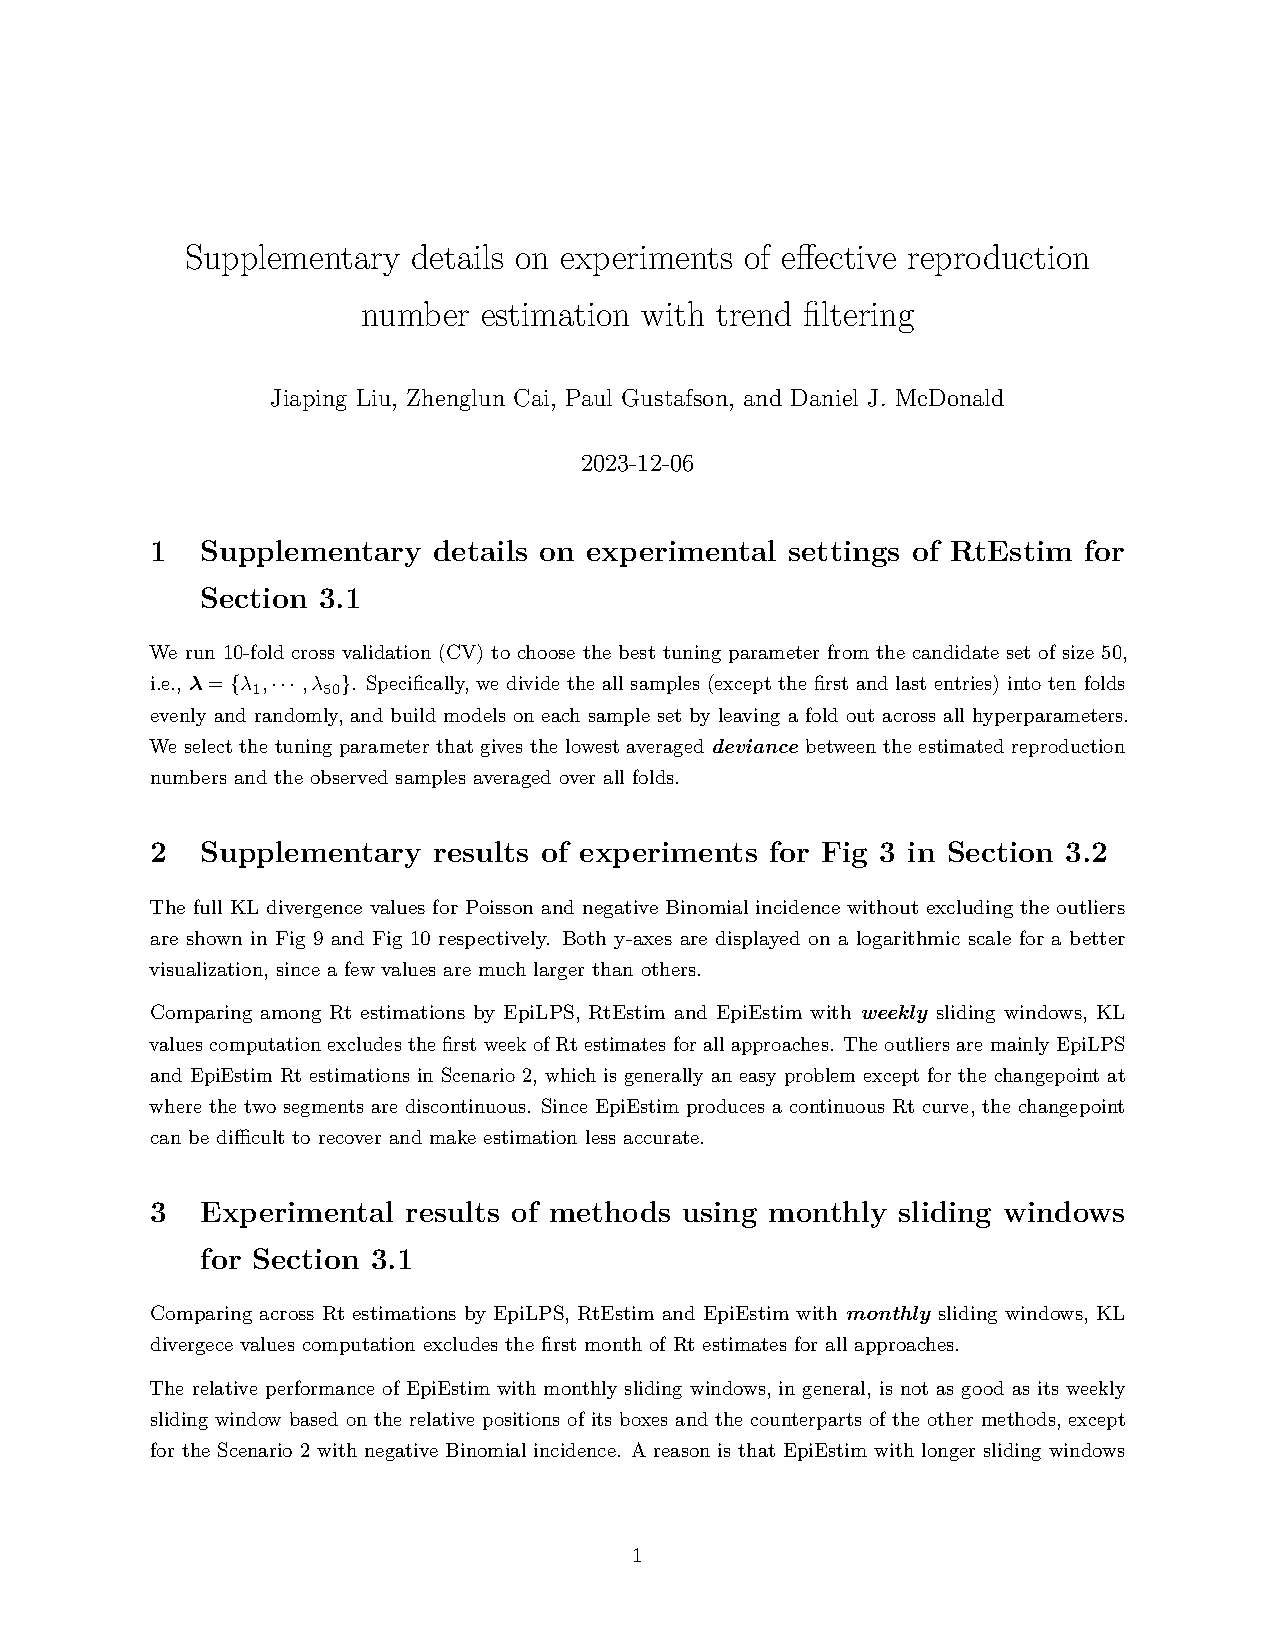
\includepdf[pages=-]{src/supp.pdf}

\end{document}
